
\documentclass{article} % For LaTeX2e
% style file edited by AI to be more preprint
\usepackage{iclr2026_conference_preprint,times}

% Optional math commands from https://github.com/goodfeli/dlbook_notation.
%%%%% NEW MATH DEFINITIONS %%%%%

\usepackage{amsmath,amsfonts,bm}

% Mark sections of captions for referring to divisions of figures
\newcommand{\figleft}{{\em (Left)}}
\newcommand{\figcenter}{{\em (Center)}}
\newcommand{\figright}{{\em (Right)}}
\newcommand{\figtop}{{\em (Top)}}
\newcommand{\figbottom}{{\em (Bottom)}}
\newcommand{\captiona}{{\em (a)}}
\newcommand{\captionb}{{\em (b)}}
\newcommand{\captionc}{{\em (c)}}
\newcommand{\captiond}{{\em (d)}}

% Highlight a newly defined term
\newcommand{\newterm}[1]{{\bf #1}}


% Figure reference, lower-case.
\def\figref#1{figure~\ref{#1}}
% Figure reference, capital. For start of sentence
\def\Figref#1{Figure~\ref{#1}}
\def\twofigref#1#2{figures \ref{#1} and \ref{#2}}
\def\quadfigref#1#2#3#4{figures \ref{#1}, \ref{#2}, \ref{#3} and \ref{#4}}
% Section reference, lower-case.
\def\secref#1{section~\ref{#1}}
% Section reference, capital.
\def\Secref#1{Section~\ref{#1}}
% Reference to two sections.
\def\twosecrefs#1#2{sections \ref{#1} and \ref{#2}}
% Reference to three sections.
\def\secrefs#1#2#3{sections \ref{#1}, \ref{#2} and \ref{#3}}
% Reference to an equation, lower-case.
\def\eqref#1{equation~\ref{#1}}
% Reference to an equation, upper case
\def\Eqref#1{Equation~\ref{#1}}
% A raw reference to an equation---avoid using if possible
\def\plaineqref#1{\ref{#1}}
% Reference to a chapter, lower-case.
\def\chapref#1{chapter~\ref{#1}}
% Reference to an equation, upper case.
\def\Chapref#1{Chapter~\ref{#1}}
% Reference to a range of chapters
\def\rangechapref#1#2{chapters\ref{#1}--\ref{#2}}
% Reference to an algorithm, lower-case.
\def\algref#1{algorithm~\ref{#1}}
% Reference to an algorithm, upper case.
\def\Algref#1{Algorithm~\ref{#1}}
\def\twoalgref#1#2{algorithms \ref{#1} and \ref{#2}}
\def\Twoalgref#1#2{Algorithms \ref{#1} and \ref{#2}}
% Reference to a part, lower case
\def\partref#1{part~\ref{#1}}
% Reference to a part, upper case
\def\Partref#1{Part~\ref{#1}}
\def\twopartref#1#2{parts \ref{#1} and \ref{#2}}

\def\ceil#1{\lceil #1 \rceil}
\def\floor#1{\lfloor #1 \rfloor}
\def\1{\bm{1}}
\newcommand{\train}{\mathcal{D}}
\newcommand{\valid}{\mathcal{D_{\mathrm{valid}}}}
\newcommand{\test}{\mathcal{D_{\mathrm{test}}}}

\def\eps{{\epsilon}}


% Random variables
\def\reta{{\textnormal{$\eta$}}}
\def\ra{{\textnormal{a}}}
\def\rb{{\textnormal{b}}}
\def\rc{{\textnormal{c}}}
\def\rd{{\textnormal{d}}}
\def\re{{\textnormal{e}}}
\def\rf{{\textnormal{f}}}
\def\rg{{\textnormal{g}}}
\def\rh{{\textnormal{h}}}
\def\ri{{\textnormal{i}}}
\def\rj{{\textnormal{j}}}
\def\rk{{\textnormal{k}}}
\def\rl{{\textnormal{l}}}
% rm is already a command, just don't name any random variables m
\def\rn{{\textnormal{n}}}
\def\ro{{\textnormal{o}}}
\def\rp{{\textnormal{p}}}
\def\rq{{\textnormal{q}}}
\def\rr{{\textnormal{r}}}
\def\rs{{\textnormal{s}}}
\def\rt{{\textnormal{t}}}
\def\ru{{\textnormal{u}}}
\def\rv{{\textnormal{v}}}
\def\rw{{\textnormal{w}}}
\def\rx{{\textnormal{x}}}
\def\ry{{\textnormal{y}}}
\def\rz{{\textnormal{z}}}

% Random vectors
\def\rvepsilon{{\mathbf{\epsilon}}}
\def\rvtheta{{\mathbf{\theta}}}
\def\rva{{\mathbf{a}}}
\def\rvb{{\mathbf{b}}}
\def\rvc{{\mathbf{c}}}
\def\rvd{{\mathbf{d}}}
\def\rve{{\mathbf{e}}}
\def\rvf{{\mathbf{f}}}
\def\rvg{{\mathbf{g}}}
\def\rvh{{\mathbf{h}}}
\def\rvu{{\mathbf{i}}}
\def\rvj{{\mathbf{j}}}
\def\rvk{{\mathbf{k}}}
\def\rvl{{\mathbf{l}}}
\def\rvm{{\mathbf{m}}}
\def\rvn{{\mathbf{n}}}
\def\rvo{{\mathbf{o}}}
\def\rvp{{\mathbf{p}}}
\def\rvq{{\mathbf{q}}}
\def\rvr{{\mathbf{r}}}
\def\rvs{{\mathbf{s}}}
\def\rvt{{\mathbf{t}}}
\def\rvu{{\mathbf{u}}}
\def\rvv{{\mathbf{v}}}
\def\rvw{{\mathbf{w}}}
\def\rvx{{\mathbf{x}}}
\def\rvy{{\mathbf{y}}}
\def\rvz{{\mathbf{z}}}

% Elements of random vectors
\def\erva{{\textnormal{a}}}
\def\ervb{{\textnormal{b}}}
\def\ervc{{\textnormal{c}}}
\def\ervd{{\textnormal{d}}}
\def\erve{{\textnormal{e}}}
\def\ervf{{\textnormal{f}}}
\def\ervg{{\textnormal{g}}}
\def\ervh{{\textnormal{h}}}
\def\ervi{{\textnormal{i}}}
\def\ervj{{\textnormal{j}}}
\def\ervk{{\textnormal{k}}}
\def\ervl{{\textnormal{l}}}
\def\ervm{{\textnormal{m}}}
\def\ervn{{\textnormal{n}}}
\def\ervo{{\textnormal{o}}}
\def\ervp{{\textnormal{p}}}
\def\ervq{{\textnormal{q}}}
\def\ervr{{\textnormal{r}}}
\def\ervs{{\textnormal{s}}}
\def\ervt{{\textnormal{t}}}
\def\ervu{{\textnormal{u}}}
\def\ervv{{\textnormal{v}}}
\def\ervw{{\textnormal{w}}}
\def\ervx{{\textnormal{x}}}
\def\ervy{{\textnormal{y}}}
\def\ervz{{\textnormal{z}}}

% Random matrices
\def\rmA{{\mathbf{A}}}
\def\rmB{{\mathbf{B}}}
\def\rmC{{\mathbf{C}}}
\def\rmD{{\mathbf{D}}}
\def\rmE{{\mathbf{E}}}
\def\rmF{{\mathbf{F}}}
\def\rmG{{\mathbf{G}}}
\def\rmH{{\mathbf{H}}}
\def\rmI{{\mathbf{I}}}
\def\rmJ{{\mathbf{J}}}
\def\rmK{{\mathbf{K}}}
\def\rmL{{\mathbf{L}}}
\def\rmM{{\mathbf{M}}}
\def\rmN{{\mathbf{N}}}
\def\rmO{{\mathbf{O}}}
\def\rmP{{\mathbf{P}}}
\def\rmQ{{\mathbf{Q}}}
\def\rmR{{\mathbf{R}}}
\def\rmS{{\mathbf{S}}}
\def\rmT{{\mathbf{T}}}
\def\rmU{{\mathbf{U}}}
\def\rmV{{\mathbf{V}}}
\def\rmW{{\mathbf{W}}}
\def\rmX{{\mathbf{X}}}
\def\rmY{{\mathbf{Y}}}
\def\rmZ{{\mathbf{Z}}}

% Elements of random matrices
\def\ermA{{\textnormal{A}}}
\def\ermB{{\textnormal{B}}}
\def\ermC{{\textnormal{C}}}
\def\ermD{{\textnormal{D}}}
\def\ermE{{\textnormal{E}}}
\def\ermF{{\textnormal{F}}}
\def\ermG{{\textnormal{G}}}
\def\ermH{{\textnormal{H}}}
\def\ermI{{\textnormal{I}}}
\def\ermJ{{\textnormal{J}}}
\def\ermK{{\textnormal{K}}}
\def\ermL{{\textnormal{L}}}
\def\ermM{{\textnormal{M}}}
\def\ermN{{\textnormal{N}}}
\def\ermO{{\textnormal{O}}}
\def\ermP{{\textnormal{P}}}
\def\ermQ{{\textnormal{Q}}}
\def\ermR{{\textnormal{R}}}
\def\ermS{{\textnormal{S}}}
\def\ermT{{\textnormal{T}}}
\def\ermU{{\textnormal{U}}}
\def\ermV{{\textnormal{V}}}
\def\ermW{{\textnormal{W}}}
\def\ermX{{\textnormal{X}}}
\def\ermY{{\textnormal{Y}}}
\def\ermZ{{\textnormal{Z}}}

% Vectors
\def\vzero{{\bm{0}}}
\def\vone{{\bm{1}}}
\def\vmu{{\bm{\mu}}}
\def\vtheta{{\bm{\theta}}}
\def\va{{\bm{a}}}
\def\vb{{\bm{b}}}
\def\vc{{\bm{c}}}
\def\vd{{\bm{d}}}
\def\ve{{\bm{e}}}
\def\vf{{\bm{f}}}
\def\vg{{\bm{g}}}
\def\vh{{\bm{h}}}
\def\vi{{\bm{i}}}
\def\vj{{\bm{j}}}
\def\vk{{\bm{k}}}
\def\vl{{\bm{l}}}
\def\vm{{\bm{m}}}
\def\vn{{\bm{n}}}
\def\vo{{\bm{o}}}
\def\vp{{\bm{p}}}
\def\vq{{\bm{q}}}
\def\vr{{\bm{r}}}
\def\vs{{\bm{s}}}
\def\vt{{\bm{t}}}
\def\vu{{\bm{u}}}
\def\vv{{\bm{v}}}
\def\vw{{\bm{w}}}
\def\vx{{\bm{x}}}
\def\vy{{\bm{y}}}
\def\vz{{\bm{z}}}

% Elements of vectors
\def\evalpha{{\alpha}}
\def\evbeta{{\beta}}
\def\evepsilon{{\epsilon}}
\def\evlambda{{\lambda}}
\def\evomega{{\omega}}
\def\evmu{{\mu}}
\def\evpsi{{\psi}}
\def\evsigma{{\sigma}}
\def\evtheta{{\theta}}
\def\eva{{a}}
\def\evb{{b}}
\def\evc{{c}}
\def\evd{{d}}
\def\eve{{e}}
\def\evf{{f}}
\def\evg{{g}}
\def\evh{{h}}
\def\evi{{i}}
\def\evj{{j}}
\def\evk{{k}}
\def\evl{{l}}
\def\evm{{m}}
\def\evn{{n}}
\def\evo{{o}}
\def\evp{{p}}
\def\evq{{q}}
\def\evr{{r}}
\def\evs{{s}}
\def\evt{{t}}
\def\evu{{u}}
\def\evv{{v}}
\def\evw{{w}}
\def\evx{{x}}
\def\evy{{y}}
\def\evz{{z}}

% Matrix
\def\mA{{\bm{A}}}
\def\mB{{\bm{B}}}
\def\mC{{\bm{C}}}
\def\mD{{\bm{D}}}
\def\mE{{\bm{E}}}
\def\mF{{\bm{F}}}
\def\mG{{\bm{G}}}
\def\mH{{\bm{H}}}
\def\mI{{\bm{I}}}
\def\mJ{{\bm{J}}}
\def\mK{{\bm{K}}}
\def\mL{{\bm{L}}}
\def\mM{{\bm{M}}}
\def\mN{{\bm{N}}}
\def\mO{{\bm{O}}}
\def\mP{{\bm{P}}}
\def\mQ{{\bm{Q}}}
\def\mR{{\bm{R}}}
\def\mS{{\bm{S}}}
\def\mT{{\bm{T}}}
\def\mU{{\bm{U}}}
\def\mV{{\bm{V}}}
\def\mW{{\bm{W}}}
\def\mX{{\bm{X}}}
\def\mY{{\bm{Y}}}
\def\mZ{{\bm{Z}}}
\def\mBeta{{\bm{\beta}}}
\def\mPhi{{\bm{\Phi}}}
\def\mLambda{{\bm{\Lambda}}}
\def\mSigma{{\bm{\Sigma}}}

% Tensor
\DeclareMathAlphabet{\mathsfit}{\encodingdefault}{\sfdefault}{m}{sl}
\SetMathAlphabet{\mathsfit}{bold}{\encodingdefault}{\sfdefault}{bx}{n}
\newcommand{\tens}[1]{\bm{\mathsfit{#1}}}
\def\tA{{\tens{A}}}
\def\tB{{\tens{B}}}
\def\tC{{\tens{C}}}
\def\tD{{\tens{D}}}
\def\tE{{\tens{E}}}
\def\tF{{\tens{F}}}
\def\tG{{\tens{G}}}
\def\tH{{\tens{H}}}
\def\tI{{\tens{I}}}
\def\tJ{{\tens{J}}}
\def\tK{{\tens{K}}}
\def\tL{{\tens{L}}}
\def\tM{{\tens{M}}}
\def\tN{{\tens{N}}}
\def\tO{{\tens{O}}}
\def\tP{{\tens{P}}}
\def\tQ{{\tens{Q}}}
\def\tR{{\tens{R}}}
\def\tS{{\tens{S}}}
\def\tT{{\tens{T}}}
\def\tU{{\tens{U}}}
\def\tV{{\tens{V}}}
\def\tW{{\tens{W}}}
\def\tX{{\tens{X}}}
\def\tY{{\tens{Y}}}
\def\tZ{{\tens{Z}}}


% Graph
\def\gA{{\mathcal{A}}}
\def\gB{{\mathcal{B}}}
\def\gC{{\mathcal{C}}}
\def\gD{{\mathcal{D}}}
\def\gE{{\mathcal{E}}}
\def\gF{{\mathcal{F}}}
\def\gG{{\mathcal{G}}}
\def\gH{{\mathcal{H}}}
\def\gI{{\mathcal{I}}}
\def\gJ{{\mathcal{J}}}
\def\gK{{\mathcal{K}}}
\def\gL{{\mathcal{L}}}
\def\gM{{\mathcal{M}}}
\def\gN{{\mathcal{N}}}
\def\gO{{\mathcal{O}}}
\def\gP{{\mathcal{P}}}
\def\gQ{{\mathcal{Q}}}
\def\gR{{\mathcal{R}}}
\def\gS{{\mathcal{S}}}
\def\gT{{\mathcal{T}}}
\def\gU{{\mathcal{U}}}
\def\gV{{\mathcal{V}}}
\def\gW{{\mathcal{W}}}
\def\gX{{\mathcal{X}}}
\def\gY{{\mathcal{Y}}}
\def\gZ{{\mathcal{Z}}}

% Sets
\def\sA{{\mathbb{A}}}
\def\sB{{\mathbb{B}}}
\def\sC{{\mathbb{C}}}
\def\sD{{\mathbb{D}}}
% Don't use a set called E, because this would be the same as our symbol
% for expectation.
\def\sF{{\mathbb{F}}}
\def\sG{{\mathbb{G}}}
\def\sH{{\mathbb{H}}}
\def\sI{{\mathbb{I}}}
\def\sJ{{\mathbb{J}}}
\def\sK{{\mathbb{K}}}
\def\sL{{\mathbb{L}}}
\def\sM{{\mathbb{M}}}
\def\sN{{\mathbb{N}}}
\def\sO{{\mathbb{O}}}
\def\sP{{\mathbb{P}}}
\def\sQ{{\mathbb{Q}}}
\def\sR{{\mathbb{R}}}
\def\sS{{\mathbb{S}}}
\def\sT{{\mathbb{T}}}
\def\sU{{\mathbb{U}}}
\def\sV{{\mathbb{V}}}
\def\sW{{\mathbb{W}}}
\def\sX{{\mathbb{X}}}
\def\sY{{\mathbb{Y}}}
\def\sZ{{\mathbb{Z}}}

% Entries of a matrix
\def\emLambda{{\Lambda}}
\def\emA{{A}}
\def\emB{{B}}
\def\emC{{C}}
\def\emD{{D}}
\def\emE{{E}}
\def\emF{{F}}
\def\emG{{G}}
\def\emH{{H}}
\def\emI{{I}}
\def\emJ{{J}}
\def\emK{{K}}
\def\emL{{L}}
\def\emM{{M}}
\def\emN{{N}}
\def\emO{{O}}
\def\emP{{P}}
\def\emQ{{Q}}
\def\emR{{R}}
\def\emS{{S}}
\def\emT{{T}}
\def\emU{{U}}
\def\emV{{V}}
\def\emW{{W}}
\def\emX{{X}}
\def\emY{{Y}}
\def\emZ{{Z}}
\def\emSigma{{\Sigma}}

% entries of a tensor
% Same font as tensor, without \bm wrapper
\newcommand{\etens}[1]{\mathsfit{#1}}
\def\etLambda{{\etens{\Lambda}}}
\def\etA{{\etens{A}}}
\def\etB{{\etens{B}}}
\def\etC{{\etens{C}}}
\def\etD{{\etens{D}}}
\def\etE{{\etens{E}}}
\def\etF{{\etens{F}}}
\def\etG{{\etens{G}}}
\def\etH{{\etens{H}}}
\def\etI{{\etens{I}}}
\def\etJ{{\etens{J}}}
\def\etK{{\etens{K}}}
\def\etL{{\etens{L}}}
\def\etM{{\etens{M}}}
\def\etN{{\etens{N}}}
\def\etO{{\etens{O}}}
\def\etP{{\etens{P}}}
\def\etQ{{\etens{Q}}}
\def\etR{{\etens{R}}}
\def\etS{{\etens{S}}}
\def\etT{{\etens{T}}}
\def\etU{{\etens{U}}}
\def\etV{{\etens{V}}}
\def\etW{{\etens{W}}}
\def\etX{{\etens{X}}}
\def\etY{{\etens{Y}}}
\def\etZ{{\etens{Z}}}

% The true underlying data generating distribution
\newcommand{\pdata}{p_{\rm{data}}}
% The empirical distribution defined by the training set
\newcommand{\ptrain}{\hat{p}_{\rm{data}}}
\newcommand{\Ptrain}{\hat{P}_{\rm{data}}}
% The model distribution
\newcommand{\pmodel}{p_{\rm{model}}}
\newcommand{\Pmodel}{P_{\rm{model}}}
\newcommand{\ptildemodel}{\tilde{p}_{\rm{model}}}
% Stochastic autoencoder distributions
\newcommand{\pencode}{p_{\rm{encoder}}}
\newcommand{\pdecode}{p_{\rm{decoder}}}
\newcommand{\precons}{p_{\rm{reconstruct}}}

\newcommand{\laplace}{\mathrm{Laplace}} % Laplace distribution

\newcommand{\E}{\mathbb{E}}
\newcommand{\Ls}{\mathcal{L}}
\newcommand{\R}{\mathbb{R}}
\newcommand{\emp}{\tilde{p}}
\newcommand{\lr}{\alpha}
\newcommand{\reg}{\lambda}
\newcommand{\rect}{\mathrm{rectifier}}
\newcommand{\softmax}{\mathrm{softmax}}
\newcommand{\sigmoid}{\sigma}
\newcommand{\softplus}{\zeta}
\newcommand{\KL}{D_{\mathrm{KL}}}
\newcommand{\Var}{\mathrm{Var}}
\newcommand{\standarderror}{\mathrm{SE}}
\newcommand{\Cov}{\mathrm{Cov}}
% Wolfram Mathworld says $L^2$ is for function spaces and $\ell^2$ is for vectors
% But then they seem to use $L^2$ for vectors throughout the site, and so does
% wikipedia.
\newcommand{\normlzero}{L^0}
\newcommand{\normlone}{L^1}
\newcommand{\normltwo}{L^2}
\newcommand{\normlp}{L^p}
\newcommand{\normmax}{L^\infty}

\newcommand{\parents}{Pa} % See usage in notation.tex. Chosen to match Daphne's book.

\DeclareMathOperator*{\argmax}{arg\,max}
\DeclareMathOperator*{\argmin}{arg\,min}

\DeclareMathOperator{\sign}{sign}
\DeclareMathOperator{\Tr}{Tr}
\let\ab\allowbreak


\usepackage{hyperref}
\usepackage{url}
\usepackage{xspace}
\usepackage{booktabs}
\usepackage{siunitx}
\usepackage{float}


\title{Prediction, Filtering, and Smoothing with Neural Network Dynamics}

% Authors must not appear in the submitted version. They should be hidden
% as long as the \iclrfinalcopy macro remains commented out below.
% Non-anonymous submissions will be rejected without review.

\author{Antiquus S.~Hippocampus, Natalia Cerebro \& Amelie P. Amygdale \thanks{ Use footnote for providing further information
about author (webpage, alternative address)---\emph{not} for acknowledging
funding agencies.  Funding acknowledgements go at the end of the paper.} \\
Department of Computer Science\\    
Cranberry-Lemon University\\
Pittsburgh, PA 15213, USA \\
\texttt{\{hippo,brain,jen\}@cs.cranberry-lemon.edu} \\
\And
Ji Q. Ren \& Yevgeny LeNet \\
Department of Computational Neuroscience \\
University of the Witwatersrand \\
Joburg, South Africa \\
\texttt{\{robot,net\}@wits.ac.za} \\
\AND
Coauthor \\
Affiliation \\
Address \\
\texttt{email}
}

% The \author macro works with any number of authors. There are two commands
% used to separate the names and addresses of multiple authors: \And and \AND.
%
% Using \And between authors leaves it to \LaTeX{} to determine where to break
% the lines. Using \AND forces a linebreak at that point. So, if \LaTeX{}
% puts 3 of 4 authors names on the first line, and the last on the second
% line, try using \AND instead of \And before the third author name.

\newcommand{\fix}{\marginpar{FIX}}
\newcommand{\new}{\marginpar{NEW}}

% \iclrfinalcopy % Uncomment for camera-ready version, but NOT for submission.

\newcommand{\neuralUQ}{{\color{red} \textbf{Neural UQ}}\xspace}

\usepackage{amsmath, amsthm, amsfonts, amssymb, mathtools, commath,
hyperref, cancel, bm}
\usepackage{algorithm,algpseudocode, algorithmicx}
\usepackage{doi, xcolor}
\newtheorem{definition}{Definition}
\newtheorem{proposition}{Proposition}
\newtheorem{conjecture}{Conjecture}
\newtheorem{theorem}{Theorem}
\newtheorem{problem}{Problem}
\newtheorem{corollary}{Corollary}
\newtheorem{remark}{Remark}
\newtheorem{lemma}{Lemma}
\newtheorem{example}{Example}
\DeclareMathOperator{\trace}{\operatorname{tr}}
\DeclareMathOperator{\expect}{\mathbb{E}}
\DeclareMathOperator{\probability}{\mathbb{P}}
% \DeclareMathOperator{\Var}{\operatorname{Var}}
% \DeclareMathOperator{\Cov}{\operatorname{Cov}}

% pseudo-true
\DeclareMathOperator{\normal}{\mathrm N}
% iterated approximation, very different
\DeclareMathOperator{\Normal}{\mathrm N^*}

\begin{document}
\maketitle

\begin{abstract}
The abstract paragraph should be indented 1/2~inch (3~picas) on both left and
right-hand margins. Use 10~point type, with a vertical spacing of 11~points.
The word \textsc{Abstract} must be centered, in small caps, and in point size 12. Two
line spaces precede the abstract. The abstract must be limited to one
paragraph.
\end{abstract}

\section{Introduction}
\subsection{Background}
We begin with a syllogism.

\textbf{Premise 1.} \emph{Neural networks are effective for modeling dynamic systems.}
Because the laws of motion of mechanical systems are often continuous functions in configuration space, they are of course representable as neural networks.
(This \emph{a priori} truism has stood up to experimentation 
[\citealt{narendra_neural_1992,masri_identification_1993}].)
But to what end?
On one hand, neural networks can recover the laws of motion of a dynamic system from data for which no parametric form is known \citep{pillonetto_deep_2025}.
On the other hand, neural networks can be supervised using the numerical solution of another physical model that might prove more costly to evaluate \citep{mohajerin_multistep_2019,michalowska_neural_2024}.

\textbf{Premise 2.} \emph{Modeling dynamic systems enables prediction, filtering, and smoothing.}
Born in the late 20th century, these now-classic problems deal with estimating the latent state of a partially observed Markov model (presented dutifully in the next section),
for example, tracking and predicting the ballistic motion of a point mass (such as a golf ball) on the basis of noisy measurements such as radar,
 or estimating one's own location by fusing 
inertial sensors and satellite navigation.
Sundry applications include human physiology forecasting \cite{albers_interpretable_2023}, pandemic surveillance \cite{alsaggaf_nonlinear_2024}, and latent macroeconomic variables \cite{burmeister_kalman_1982}.
\citet{kalman_new_1961} and \citet{luenberger_observing_1964} stated and solved the filtering problem for linear dynamic system models.
For nonlinear models, the playing field for how to generalize the Kalman Filter is wide and hotly contested.
It is currently occupied by the Extended, Unscented, and countless other Kalman Filters that claim to handle nonlinearity more faithfully \citep{sarkka_bayesian_2023,jiang_new_2025}.

\textbf{Conclusion.} \emph{Therefore, neural networks enable prediction, filtering, and smoothing.}
We are not the first to make this connection.
Existing work has embedded the neural mapping inside an general-purpose nonlinear Kalman filter such as the Extended Kalman Filter \citep{oveissi_novel_2025} or the Unscented Kalman Filter \citep{anurag_rcukf_2025}.
(Also see \citet{bai_state_2023} for an ample bibliography.)

\subsection{Foreground}
We summarize this paper's contributions in a new syllogism.

\textbf{Premise 1.} \emph{Neural networks are effective for propagating uncertainty in dynamic systems.}
This paper builds on the uncertainty propagation methodology of \neuralUQ, which finds that with the right activation function, the first two moments of a Normal distribution can be propagated exactly through a single layer of a feedforward neural network, and by extension, approximately through a deep feedforward neural network.
% % ;
% and that this Ansatz is competitive with and sometimes outperforms other moment propagation methods.
The experience of \citet{deisenroth_analytic_2009} suggests that accurate moment propagation is beneficial for Kalman filtering on models represented as Gaussian processes.
This work extends that methodology to models represented as neural networks.

\textbf{Premise 2.} \emph{Neural network uncertainty propagation enables prediction, filtering, and smoothing.}
By recasting prediction, filtering, and smoothing as alternating Gaussian conditioning with nonlinear uncertainty propagation, one can put the various Kalman filters on a common footing \citep{sarkka_bayesian_2023,hennig_probabilistic_2022}.
In particular, the various uncertainty propagation methods benchmarked in \neuralUQ correspond to different flavors of Kalman filtering.

\textbf{Conclusion.} \emph{Therefore, analytic moment propagation through neural networks enables prediction, filtering, and smoothing} of problems hitherto believed to be intractable.
The literature exhibits a survivorship bias for nonlinear filtering and smoothing problems that are amenable to general-purpose nonlinear Kalman filters (as detailed in the Background section).
Usually, this amounts to selecting a sampling time that is small enough that the continuous-time system behaves as a linear system with slowly-varying parameters.
For example, the Lorenz system is filtered using a discretization time of 0.001 \citep{nosrati_chaotic_2011}, 0.005 \citep{dubois_data-driven_2020}, or 0.01 \cite{oveissi_novel_2025}.
Our work extends the discretization time to 1, which is on the order of a full period of the chaotic attractor.

We do not impeach the Extended, Unscented etc.~Kalman filters as unfit for purpose.
% on existing problems, our method is only an incremental improvement.
Rather, our method dramatically expands the scope of problems that can be tackled with Kalman filtering.

The bottom line is that on highly nonlinear problems, our method improves upon existing Kalman filters in both accuracy and calibration.
\begin{description}
    \item[accuracy] We show an improvement in the point prediction and estimate of the state. Qualitatively, we observe that our estimator is able to stay synchronized with the chaotic Lorenz system.
    \item[calibration] We demonstrate that confidence regions predicted by our method's state covariances have better coverage than existing Kalman filters.
    That is, 95\% confidence regions for the state should contain the true state roughly 95\% of the time.
    This enables risk-aware decision making for optimally trading between safety and performance.
\end{description}

\section{Notation}
When \(\sigma:\mathbb R \to \mathbb R\) is a neural network activation function, \(\sigma (x)\) for \(x \in \mathbb{R}^n\) is applied elementwise.

Uncertainty propagation notation follows that of \neuralUQ.
If \(X\) is a square-integrable random vector, the notation \(\normal X\) refers to a random variable having distribution \(\mathcal N(\expect X, \Cov X)\).
If \(f\) is a neural network, the notation \(\Normal f(X)\) is a Normal random variable in which the normality approximation is applied layer-by-layer as in the analytic propagation method of \neuralUQ.

% The variance-covariance matrix of a random vector \(X\) is \(\Var X = \expect(X - \expect X)(X - \expect X)^\intercal\).

% Generally, lowercase random variables \(x_t\) refer to a realization of a stochastic process.
% State dynamics \(x_{t} = F(x_{t-1}) +
% \eta_t\) are ``strong,'' i.e.~hold almost surely.

% Generally, uppercase random variables \(X_t\) refer to probability laws.
% Statements such as \(X_t = F(X_{t-1})\) are ``weak'' and denote propagation of uncertainty (the
% approximation of which is a key comparison in this paper): \(X_t\)
% is the distribution of \(F(X_{t-1})\).
% In expressions such as \(H(X_t) + \mathcal N(0, R)\), we mean that
% the noise term is independent of all other randomness.

The comma \(,\) is a higher-order function:
if \(x \mapsto f(x)\) and \(x \mapsto g(x)\) are functions, then \((f
, g)\) is the function \(x \mapsto (f(x), g(x))\).

The direct sum of two square matrices \(A\) and \(B\) is denoted by
\(A \oplus B\) and refers to the block-diagonal matrix \(A \oplus B =
  \begin{pmatrix} A & 0 \\ 0 & B
\end{pmatrix}\).

In algorithmic pseudocode, a \emph{Function} is a pure function in
the mathematical or functional
programming sense.
In particular, the variable names are meaningless placeholders.
\(f(x) = x^2\) defines the same function as \(f(y) = y^2\).
A \emph{Procedure} is code that results ``side effects.''
Inside a procedure, the variable names are meaningful and refer to
the same variables used to pose an algorithmic problem.



\section{Problem statement}
A dynamic system is described by
\begin{subequations}
  \label{eq:dynamic-system}
  \begin{align}
    x_0 &\sim \mathcal{N}(\mu_0, \Sigma_0) \\
    x_t &= F(x_{t-1}, u_t) + \eta_t, &\eta_t &\sim \mathcal{N}(0, Q)
    & \forall t &\in \cbr{1 \ldots T}\\
    y_t &= H(x_t, u_t) + \epsilon_t, &\epsilon_t &\sim \mathcal{N}(0,
    R) & \forall t &\in \cbr{1 \ldots T}
  \end{align}
\end{subequations}
where \(x_t \in \mathbb{R}^{n_x}\) is the state, \(u_t \in \mathbb
R^{n_u}\) is the input, and \(y_t \in \mathbb{R}^{n_y}\) is the output.
The random variables \(x_0\), \(\{\eta_t\}_{t=1}^T\), and
\(\{\epsilon_t\}_{t=1}^T\) are independent.

This model motivates three problems.
\begin{problem}[Prediction]\label{problem:prediction}
  Given \(\{u_s\}_{s=0}^{t-1}\) and \(\{y_s\}_{s=1}^{t-1}\), predict
  \(x_t\) and \(y_t\) as a joint distribution \((\hat X_{t \mid t-1},
  \hat Y_{t \mid t-1})\).
\end{problem}

\begin{problem}[Filtering]\label{problem:filtering}
  Given \(\{u_s\}_{s=0}^{t}\) and \(\{y_s\}_{s=1}^t\), estimate
  \(\hat X_{t \mid t}\).
\end{problem}

\begin{problem}[Smoothing]\label{problem:smoothing}
  Given \(\{u_s\}_{s=0}^T\) and \(\{y_s\}_{s=1}^T\), estimate \(\hat X_{t \mid T}\).
\end{problem}

In the case that \(F\) and \(H\) are linear functions,
the predictive and posterior distributions arising in these problems are Normal and can be computed analytically by recursion across time steps.
However, in our case, \(F\) and \(H\) are nonlinear functions.
We follow the approach of Assumed Density Filtering \cite{deisenroth_analytic_2009}, 
which re-imposes Normality assumptions on nonlinearly transformed Normal variables.
The Kalman filter Alg.~\ref{alg:kalman-filter} solves the prediction
and filtering problems by a forward recursion, and the
Rauch-Tung-Striebel smoother Alg.~\ref{alg:rts-smoother} solves the
smoothing problem by a backward recursion.
We have stylized these algorithms (cf.~\citealt[Algorithms~5.3--4, 38.1--2]{hennig_probabilistic_2022}) in order to make a common platform for the varieties of Assumed Density Filtering, which can be seen as different implementations of the ``\(\normal\)'' operator.

\begin{algorithm}
  \caption{
    \label{alg:kalman-filter}
    General Kalman algorithm for recursive \textbf{prediction} (problem
    \ref{problem:prediction}) and \textbf{filtering} (problem
  \ref{problem:filtering})}
  \begin{algorithmic}[1]
    \Require State transition function \(F\) and observation model \(H\)
    \Require State covariance \(Q\) and and observation covariance \(R\)
    \Function{Predict}{$X, u$}
    \State
    \(X' \gets \normal F(X, u) + \mathcal{N}(0, Q)\)
    \Comment{Propagate \(X\) through state transition}
    \State
    \(((X', u), Y') \gets\normal (\text{id}, H)(X', u) +
    \mathcal{N}(0, 0_{n_x} \oplus R)\)
    \Comment{Propagate \(X'\) through observation model}
    \State\Return \((X', Y')\)
    \Comment{Joint distribution of next state and next output}
    \EndFunction
    \Function{Update}{$(X, Y), y$}
    \State
    \((X', y) \gets\) conditional distribution of \((X,Y)\)
    given \(Y=y\)
    \Comment{Apply Bayes' rule}
    \State\Return \(X'\)
    \EndFunction
    \Procedure{Filter}{$u_1, \ldots, u_t, y_1, \ldots, y_t$}
    \State \(\hat X_{0 \mid 0} \gets \mathcal{N}(\mu_0, \Sigma_0)\)
    \For{$k \in \cbr{1 \ldots t}$}
    \State \( (\hat X_{k \mid k-1}, \hat Y_{k \mid k-1})
    \gets \textsc{Predict}(\hat X_{k-1 \mid k-1}, u_k) \)
    \Comment{Solution to problem \ref{problem:prediction}}
    \State \( \hat X_{k \mid k}  \gets \textsc{Update}((\hat
    X_{k \mid k-1}, \hat Y_{k \mid k-1}), y_k) \)
    \Comment{Solution to problem \ref{problem:filtering}}
    \EndFor
    \EndProcedure
  \end{algorithmic}
\end{algorithm}

\begin{algorithm}
  \caption{
    \label{alg:rts-smoother}
    General RTS algorithm for recursive \textbf{smoothing} (problem
  \ref{problem:smoothing})}
  \begin{algorithmic}[1]
    \Require State transition function \(F\)
    \Require State covariance \(Q\)
    \Function{Predict}{$X, u$}
    \State
    \(((X, u), X') \gets \normal (\text{id} , F)(X, u) +
    \mathcal{N}(0, 0 \oplus Q)\)
    \Comment{Propagate \(X\) through state transition}
    \State\Return \((X, X')\)
    \Comment{Joint distribution of current state and next state}
    \EndFunction
    \Function{Update}{$(X, X'), X''$}
    \State
    \((X, X'') \gets\) conditional distribution of
    \((X,X')\) given \(X' = X''\)
    \Comment{Apply Bayes' rule}
    \State\Return \(X\)
    \EndFunction
    \Procedure{Smooth}{$u_1, \ldots, u_T, y_1, \ldots, y_T$}
    \State \(\{\hat X_{k|k}\}_{k=1}^T \gets
    \textsc{Filter}(u_1, \ldots, u_T, y_1, \ldots, y_T)\)
    \For{$k \in \cbr{T-1 \ldots 0}$}
    \State \( (\hat X_{k|k}, \hat X_{k+1|k}) \gets
    \textsc{Predict}(\hat X_{k \mid k}, u_{k+1}) \)
    \State \( \hat X_{k|T} \gets \textsc{Update}((\hat
    X_{k|k}, \hat X_{k+1|k}), \hat X_{k|T}) \)
    \Comment{Solution to problem \ref{problem:smoothing}}
    \EndFor
    \EndProcedure
  \end{algorithmic}
\end{algorithm}

\section{Neural networks}
Our convention for neural networks follows \neuralUQ, whose definitions we repeat for convenience:

\begin{definition}
    \label{def:layer-function}
    A layer function is a function \(g:\mathbb R^n \times \mathbb R^{m \times n} \times \mathbb R^m \times \mathbb R^{m \times n} \times \mathbb R^m \to \mathbb R^m\) defined by \(g(x; A, b, C, d) = \sigma(A x + b) + C x + d\), where \(A \in \mathbb R^{m \times n}, b \in \mathbb R^m, C \in \mathbb R^{m \times n}, d \in \mathbb R^m\) are parameters.
\end{definition}

\begin{definition}
    \label{def:neural-network}
    A neural network with \(\ell \) layers is the function \(f: \mathbb R^{n_x} \to \mathbb R^{n_y}\) defined by
    \begin{align*}
        f(x) &= f^\ell(x) \\
        f^k(x) &= g(f^{k-1}(x); A^k, b^k, C^k, d^k) & \forall k &\in \cbr{1 \ldots \ell} \\
        f^0(x) &= x
    \end{align*}
\end{definition}

The four-parameter \((A, b, C, d)\) layer function is more general than customary.
This generality allows for certain possibilities such as residual networks (\(C=I\), \(d=0\)).
In the context of the Kalman and RTS algorithms, this generality affords an effortless Normal approximation of the joint distribution of a neural network's input and its output.

\subsection{The identity-augmentation operator}
Algorithms \ref{alg:kalman-filter} and \ref{alg:rts-smoother}
both invoke the identity-augmentation operator \(F \mapsto F_\text{aug}=(\text{id}, F)\) to compute the covariance between \(X\) and \(F(X)\) and the covariance between \(F(X)\) and \(F(X)\).
We construct a representation of \(F_\text{aug}\) that is itself a neural network.

\begin{lemma}
  \label{lem:augmentation}
  Neural networks defined by Def.~\ref{def:neural-network} are closed under the input coupling:
  if \(f_1\) and \(f_2\) are two neural networks with \(n\) inputs and \(\ell\) layers, then \((f_1, f_2)\) can also be parameterized by a neural network with \(n\) inputs and \(\ell\) layers.
\end{lemma}
\begin{proof}
  For \(j \in \{1, 2\}\), let \(f_j\) be defined by
  \begin{align}
    f_j(x) &= f_j^\ell(x), \\
    f_j^k(x) &= g(f_j^{k-1}(x); A_j^k, b_j^k, C_j^k, d_j^k), & k \in \cbr{1 \ldots \ell},
    \\
    f_j^0(x) &= x
  \end{align}
  Now define \(f_\text{aug} =(f_1, f_2)\) by
  \begin{align}
    f_\text{aug}(x) &= f_\text{aug}^\ell(x), \\
    f_\text{aug}^k(x) &= g(f_\text{aug}^{k-1}(x); A_\text{aug}^k, b_\text{aug}^k, C_\text{aug}^k, d_\text{aug}^k), & k \in \cbr{1 \ldots \ell},
    \\
    f_\text{aug}^0(x) &= x
  \end{align}
  where
  \begin{align}
    A_\text{aug}^1 &= \begin{pmatrix}
      A_1 \\ A_2 
    \end{pmatrix}
    &
    b_\text{aug}^1 &= \begin{pmatrix}
      b_1 \\ b_2
    \end{pmatrix}
    \\
    C_\text{aug}^1 &= \begin{pmatrix}
      C_1 \\ C_2
    \end{pmatrix}
    &
    d_\text{aug}^1 &= \begin{pmatrix}
      d_1 \\ d_2
    \end{pmatrix}
  \end{align}
  and for \(k \in \cbr{2 \ldots \ell}\),
  \begin{align}
    A_\text{aug}^k &= \begin{pmatrix}
      A_1^k & 0 \\
      0 & A_2^k
    \end{pmatrix}
    &
    b_\text{aug}^k &= \begin{pmatrix}
      b_1^k \\ b_2^k
    \end{pmatrix}
    \\
    C_\text{aug}^k &= \begin{pmatrix}
      C_1^k & 0 \\
      0 & C_2^k
    \end{pmatrix}
    &
    d_\text{aug}^k &= \begin{pmatrix}
      d_1^k \\ d_2^k
    \end{pmatrix}
  \end{align}
\end{proof}

\begin{corollary}
  If \(f\) is a neural network with \(n\) inputs and \(\ell\) layers,
  then \((\operatorname{id}, f)\) can be represented by a neural network with \(n\)
  inputs and \(\ell\) layers.
\end{corollary}
\begin{proof}
  In order to appeal to Lemma \ref{lem:augmentation}, we just have to represent the identity map as a neural network with \(\ell\) layers.
  This can be done by setting \(A^k = 0\), \(b^k = 0\), \(C^k = I\) and \(d^k = 0\) for all \(k \in \cbr{1 \ldots \ell}\).
\end{proof}

\subsection{Methods for uncertainty propagation: with application to Kalman filtering}
Let \(X\) be a multivariate Normal random variable and \(F\) a neural network following Def.~\ref{def:neural-network}.
Uncertainty propagation refers to approximating\footnote{For a deep neural network, accurate uncertainty propagation is \(\sharp\)P-hard; see \S5, \neuralUQ.} the mean and covariance matrix of \(Y = F(X)\).
It appears as the ``\(\normal\)'' operator in Alg.~\ref{alg:kalman-filter}, lines 2--3; and Alg.~\ref{alg:rts-smoother}, line 2.
The material in this section draws on \S3, \neuralUQ, and we refer to that work for more details.

This paper introduces the \textbf{\textsc{analytic} Kalman filter}, in which ``\(\normal\)'' is implemented using the layer-by-layer moment matching method introduced in \neuralUQ, which provides analytical expressions for the cases where \(\sigma\) is a Normal CDF function or a sinusoid.
\begin{definition}
    Let \(f\) be a neural network with \(\ell\) layers.
    Given \(X \sim \mathcal N(\mu, \Sigma)\), the layer-wise Gaussian approximation of \(f(X)\), denoted \(Y_\mathrm{ana} = \Normal f(X)\), is the random variable defined by
    \begin{align*}
        Y_\mathrm{ana} &=  Y^\ell\\
        Y^k &= \normal g(Y^{k-1}; A^k, b^k, C^k, d^k) & \forall k &\in \cbr{1 \ldots \ell} \\
        Y^0 &= X
    \end{align*}
\end{definition}

Inspired by \citet{huber_bayesian_2020, wagner_kalman_2022,akgul_deterministic_2025}, we define the \textbf{\textsc{mean-field} analytic Kalman filter} by assuming that neurons in the same hidden layer are independent:
\begin{align*}
  Y_\mathrm{mfa} &=  Y^\ell\\
  Y^k &= \mathcal N(\mu^k, \Sigma^k) & \forall k &\in \cbr{1 \ldots \ell} \\
  \mu^k &= \expect g(Y^{k-1}; A^k, b^k, C^k, d^k)
  \\
  \Sigma^k_{ij} &= \begin{cases}
    \sbr{\Cov g(Y^{k-1}; A^k, b^k, C^k, d^k)}_{ij}, & i=j
    \\
    0, &\text{else}
  \end{cases}
  \\
  Y^0 &= X
\end{align*}

The \textbf{\textsc{extended} Kalman filter} in works such as \citet{jiang_new_2025,oveissi_novel_2025} uses a linearization of the neural network
\citep{titensky_uncertainty_2018, nagel_kalman-bucy-informed_2022,petersen_uncertainty_2024, jungmann_analytical_2025}.

The \textbf{\textsc{unscented'95} Kalman filter} introduced in \citep{julier_new_1995,julier_new_1997,julier_new_2000} is a one-parameter family of transformations that approximate the distribution of \(X\) by \(2n +1\) point masses.

The \textbf{\textsc{unscented'02} Kalman filter} introduced in \citep{julier_scaled_2002,wan_unscented_2000} adds two additional hyperparameters.
It is more commonly used today \citep{jiang_new_2025,anurag_rcukf_2025} and is the default in off-the-shelf software \citep{ljung_unscentedkalmanfilter_2025}.

Each of these methods is also tested with the \textbf{\textsc{recalibrate}} variation in which the \textsc{Update} step (Alg..~\ref{alg:kalman-filter}) is replaced by the recalibrate/back-out procedure described in \citet[Alg.~1]{jiang_new_2025}, which claims that the \textsc{recalibrate} variation of nonlinear Kalman filtering confers a more conservative management of state uncertainty in the presence of strong nonlinearity.

We also benchmark against the \textbf{\textsc{stationary}} state estimate, which predicts a constant \(\hat x\) for all \(t\):
\begin{subequations}
\begin{align}
  \hat x_{\mathrm{stationary}} &= \mathcal N(\mu_{\mathrm{stationary}}, \Sigma_{\mathrm{stationary}})
  \\
  \mu_{\mathrm{stationary}} &= \frac{1}{T+1} \sum_{t = 0}^T x_t
  \\
  \Sigma_{\mathrm{stationary}} &= \frac{1}{T} \sum_{t = 0}^T (x_t - \mu_{\mathrm{stationary}})(x_t - \mu_{\mathrm{stationary}})^\intercal
\end{align}
\end{subequations}

\section{On the calibration of Kalman filters}
It is frequently asserted that the Gaussian posterior distributions arising from nonlinear Kalman filters and RTS smoothers contain a meaningful measure of uncertainty.
That is, if, say, a Kalman filter reports \(\hat x_{t \mid t} = \mathcal N(\mu_{t \mid t}, \Sigma_{t \mid t})\), then \(\mu_{t \mid t}\) is a good point estimate of \(x_{t \mid t}\) and \(\Sigma_{t \mid t}\) is an expression of the uncertainty in \(x_{t \mid t}\).
Simply put, a 95\% confidence set for \(x_t\) traps the true value of \(x_t\), 95\% of the time---this agreement is called \emph{calibration}.

We are unaware of any literature that attempts to validate the latter claim empirically for Kalman filtering of nonlinear dynamic systems.
The closest works are:
\begin{itemize}
  \item \citet{jiang_new_2025}, which claims that maintaining a sufficiently large \(\Sigma_{t \mid t}\) is needed to power the state update from \(\hat x_{t+1 \mid t}\) to \(\hat x_{t+1 \mid t+1}\), and
  \item \citet{deisenroth_analytic_2009}, which assesses the predictive likelihood of the true state given the filtering distribution.
  This is a step in the right direction that acknowledges that a positive matrix is not interpretable as a measure of uncertainty unless it is calibrated to the true uncertainty.
\end{itemize}

To make this notion statistically rigorous, we recall the definition of a confidence set from \citet[\S6.3.2]{wasserman_all_2004}.
(With informal reference to the Bernstein-von Mises theorem and the Bayesian frequentist literature, we elide the technical distinctions between Bayesian and frequentist confidence sets.)

\begin{definition}
Let \(C\) be a random subset of \(\mathbb R^{n}\) and let \(\theta \in \mathbb{R}^n\).
Then \(C\) is an \(\alpha\)-confidence set for \(\theta\) if
\begin{align*}
\probability\del{\theta \in C} \geq 1-\alpha.
\end{align*}
\end{definition}

In prediction, filtering, and smoothing, \(C\) is generated at every time step \(t\) using the state estimate \(\mu\) and its covariance \(\Sigma\).
Next, we define the notions of nominal coverage and actual coverage with reference to the true state \(x\).
The probabilities are interpreted as ergodic averages in \(t\) over the randomness of random state rollouts \(\{x_t\}\) as well as measurement noise entering \(\{y_t\}\).
\begin{definition}[Nominal coverage]
Suppose that \(\hat x = \mathcal N(\mu, \Sigma)\).
Then \(C\) has nominal coverage \(1 - \alpha\) if
\begin{align*}
\probability\del{\hat x \in C} \geq 1-\alpha.
\end{align*}
\end{definition}
\begin{definition}[Actual coverage]
  The set \(C\) has actual coverage \(1 - \alpha\) if
  \begin{align*}
    \probability\del{x \in C} \geq 1-\alpha.
  \end{align*}
\end{definition}

In our numerical examples, we generate the sets \(C_t\) as Mahalanobis ellipsoids, e.g.~the \((1 - \alpha)\)-confidence set for filtering is given by
\begin{align}
  C_{t\mid t} &= \set{\hat x \in \mathbb R^{n_x} \mid (\hat x - \mu_{t\mid t})^\intercal \Sigma_{t\mid t}^{-1} (\hat x - \mu_{t\mid t}) \leq F_{\chi^2(n_x)}(1 - \alpha)}
\end{align}
where \(F_{\chi^2(n_x)}\) is the cumulative distribution function of the \(\chi^2\) distribution with \(n_x\) degrees of freedom.

% Suppose that \(C_k \subset \mathbb R^{n_x}\) is a 
% It has a simple definition, which we paraphrase from \citet[Chapter~6]{wasserman_all_2004}.




\section{Example: stochastic Lorenz system}
\label{sec:stochastic-lorenz-system}
The Lorenz system is a reduced-order model of atmospheric convection that is often used is a benchmark in dynamical systems methdology.
Here, we consider the problem of estimating all three states \((x^1, x^2, x^3)\) of the Lorenz system from a sequence of noisy and temporally sparse measurements of \(x^1\).
The system of interest is the sampled stochastic Lorenz system with a deterministic initial condition.
\begin{subequations}
  \begin{align}
    x_0 &=  (-8, 4, 27) 
    \\
    x_{t} &= F(x_{t-1}, B_t) &\forall t \in \cbr{1 \ldots T}.
  \end{align}
\end{subequations}
\(B_t\) is an independent Wiener process for each \(t \in \cbr{1 \ldots T}\).
The transition function \(F\) is given by
\begin{align}
  F(x, B) &= \xi(\Delta t) \\
  \intertext{subject to}
  \xi(0) &= x \\
  \xi(t) &= \int_0^t f(\xi(s)) \dif s + \eta B(t) &\forall t \in [0, \Delta t]
\end{align}
where \(f\) is the Lorenz vector field:
\begin{subequations}
\label{eq:stochastic-lorenz-system}
\begin{align}
  f\begin{pmatrix}
    x^1\\
    x^2\\
    x^3
  \end{pmatrix}
  &= \begin{pmatrix}
    \sigma (x^2 - x^1)\\
    x^1(\rho - x^3) - x^2\\
    x^1 x^2 - \beta x^3
  \end{pmatrix}
\end{align}
\end{subequations}
where \(\sigma = 10\), \(\rho = 28\), and \(\beta = 8/3\).
The process noise standard deviation is \(\eta = 0.001\).
The measurement noise standard deviation is \(\epsilon = 0.1\).
The sampling time is \(\Delta t = 1.0\).

In order to learn the generative model \ref{eq:dynamic-system} from a
training set \(\{x_t\}_{t =0}^{T_\text{train}}\),
we learn the neural network \(F\) and process
covariance \(Q\) simultaneously by maximizing the profile likelihood:
\begin{align}
\label{eq:profile-likelihood}
  \begin{split}
    &\min_{F, Q}
    \quad
    \log \det Q
    \\
    &\text{subject to}
    \quad
    \begin{matrix}
      Q = \frac{1}{N} \sum_{t=2}^{T_\text{train}} \epsilon_t
      \epsilon_t^\intercal\\
      \epsilon_t = x_t - F(x_{t-1}, u_t)
    \end{matrix}
  \end{split}
\end{align}

The details of the implementation are given in \S\ref{sec:implementation-details}.
\subsection{Results}
The \textsc{analytic} method delivers a prediction RMSE of \(14.9\), which is on par with the RMSE of the \textsc{stationary} benchmark (Table~\ref{tab:results_rmse_pred_post}).
(The abridged discussion in this section rounds to three significant digits. For the full data, see Appendix~\ref{sec:results}).
This means that state uncertainty is so high, and the dynamics so strongly mixing, that the method's uncertainty is tantamount to that of the population of possible states.
However, the RMSE collapses significantly to \(10.0\) after seeing the next output measurement (filtering),
and to \(9.86\) after seeing the future output measurements (smoothing) (Table~\ref{tab:results_rmse_smooth}).

Even as \textsc{analytic}'s point estimates are becoming more accurate, the 95\% confidence regions become more calibrated, shrinking from \(99.2\%\) to \(98.0\%\) (Table~\ref{tab:results_coverage95_pred_post}) to \(97.8\%\) (Table~\ref{tab:results_coverage95_smooth}) actual coverage.
Similarly, the nominal 99\% confidence regions reduce in conservatism from \(99.9\%\) to \(99.6\%\) (Table~\ref{tab:results_coverage99_pred_post}) to \(99.4\%\) (Table~\ref{tab:results_coverage99_smooth}) actual coverage.

The \textsc{analytic (recal)} method has similar RMSE to \textsc{analytic}, but more conservative confidence regions---true to the claims in \citet{jiang_new_2025} that this method results in greater (in the Loewner order) covariance matrices than the vanilla Kalman update.
For example, at \(95\%\) nominal coverage, \textsc{analytic (recal)} delivers a confidence region with \(99.0\%\) actual coverage, an increase of \(1.24\%\) over \textsc{analytic}.
This means that \textsc{analytic (recal)} can be desirable if conservatism is a priority for e.g.~safety applications, but in terms of the brute statistics, it is an weaker inference method.
This is also evidenced by the fact that \textsc{analytic (recal)} has a higher average log pdf than  \textsc{analytic} (Table~\ref{tab:results_lpdf_pred_post}, Table~\ref{tab:results_lpdf_smooth}).

The \textsc{mean-field} method fails to update the state at all (Table~\ref{tab:results_rmse_pred_post}, Table~\ref{tab:results_rmse_smooth}).
This is due to the fact that state updates require cross-covariances, which are not set to zero in the mean-field method.
Therefore, even though the mean-field approximation can be useful for certain varieties of inference with neural networks, it is not a viable approximation for Kalman filtering.

The \textsc{linear} methods and all of the \textsc{unscented} methods significantly underperform \textsc{stationary} in across all three stages (prediction, filtering, smoothing) in all of the performance metrics (RMSE, coverage, log pdf).
Some striking examples: the \textsc{linear} smoother has a RMSE of 74.6, nearly five times that of \textsc{stationary}.
The \textsc{unscented'02 (recal)} filter has confidence regions of \(55.4\%\) actual coverage at \(99\%\) nominal coverage.
In many cases, we were unable to report figures of merit for \textsc{unscented'02} because the results became numerically indeterminate at 64-bit floating point precision, with covariance matrices having condition numbers on the order of \(10^{14}\).

\begin{figure}
\begin{center}
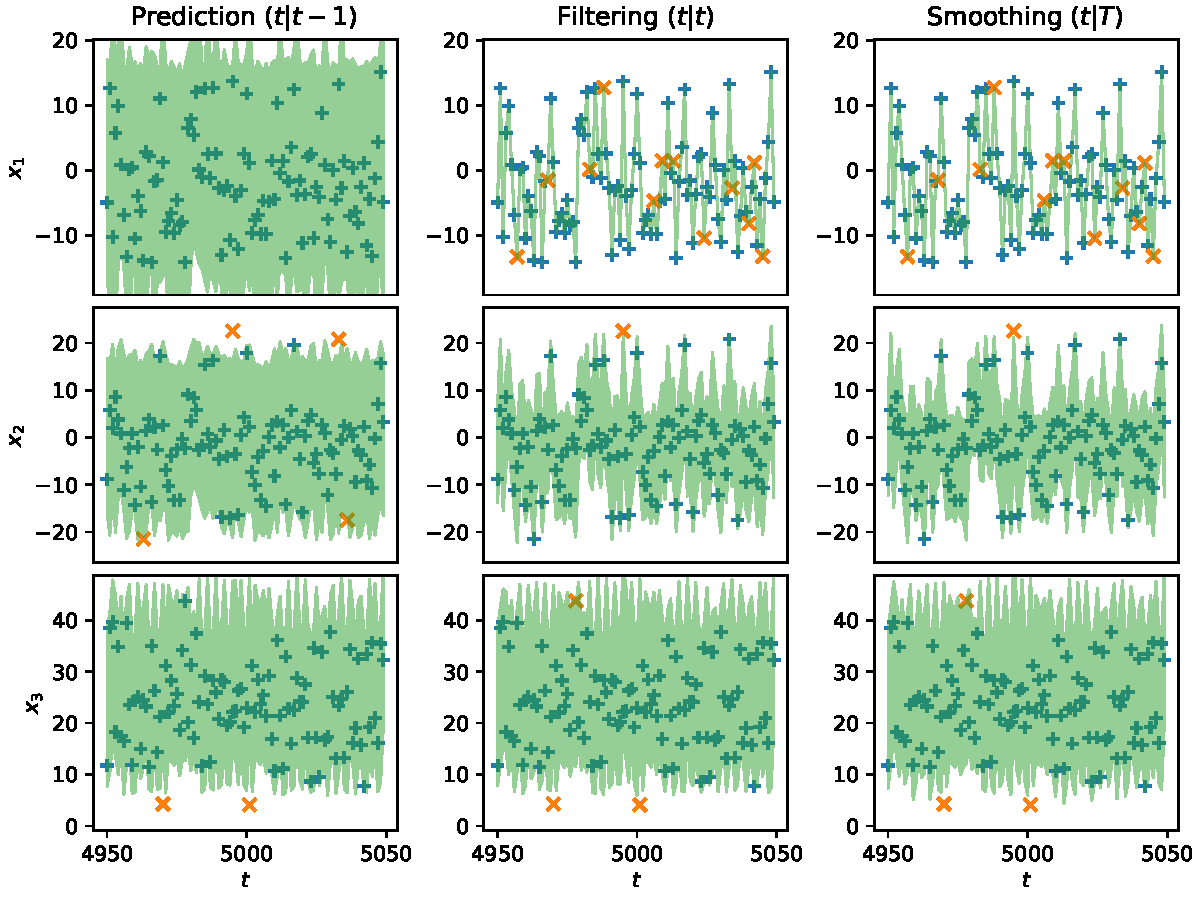
\includegraphics[width=\linewidth]{generated/trajectory/Method.ANALYTIC-Recalibrate.NO.pdf}
\end{center}
\caption{\label{fig:analytic_trajectory}Trajectory excerpt for Kalman filter \textsc{{\textsc{analytic}}}}
\end{figure}

\begin{figure}
\begin{center}
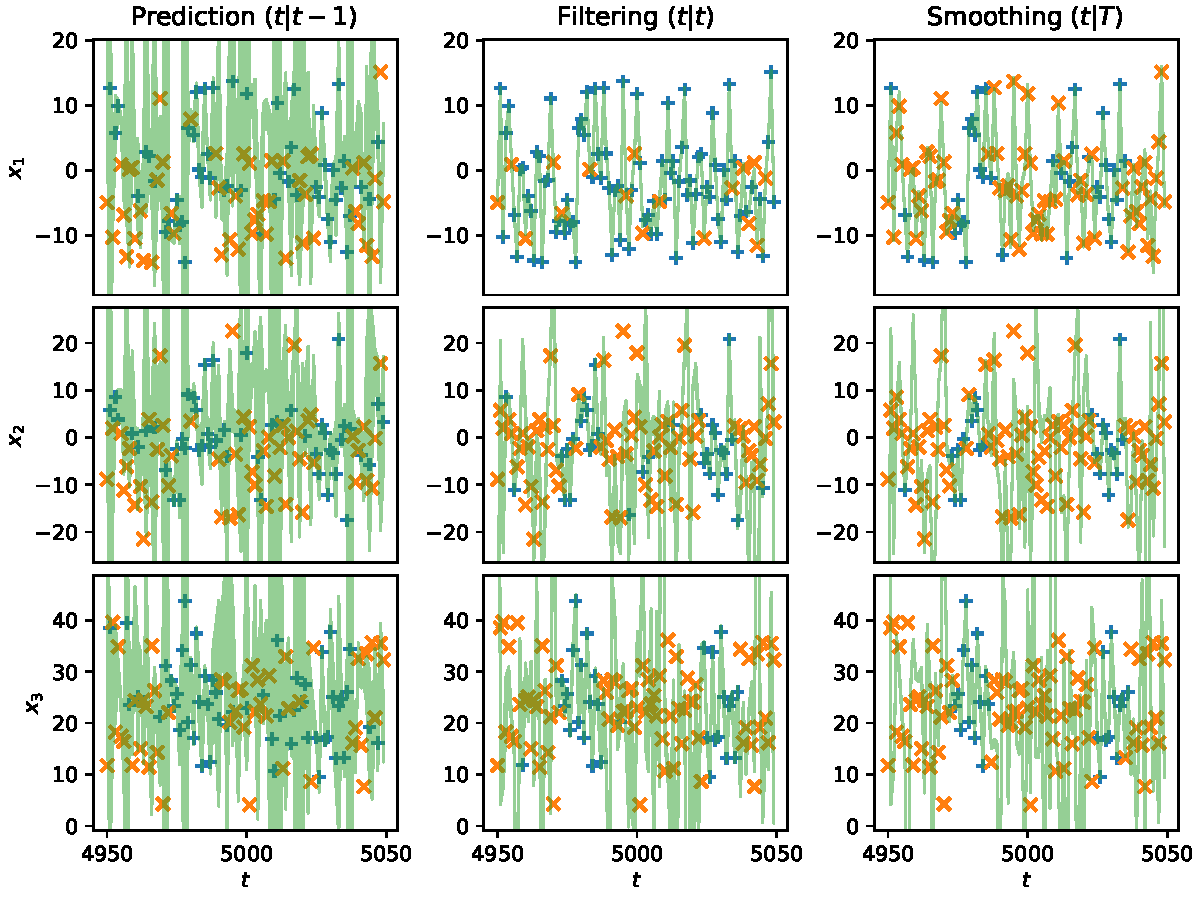
\includegraphics[width=\linewidth]{generated/trajectory/Method.LINEAR-Recalibrate.YES.pdf}
\end{center}
\caption{\label{fig:linear_trajectory}Trajectory excerpt for Kalman filter \textsc{{\textsc{linear (recal)}}}}
\end{figure}

Viewing excerpts of the state trajectories helps to explain why the non-analytic filters perform so poorly.
The confidence region of \textsc{analytic} envelops the true state (plus signs depict hits; crosses depict misses) at close to 90\% (nominal coverage) (Figure~\ref{fig:analytic_trajectory})
On the other hand, the confidence region of \textsc{linear (recal)} confidently misses the state at every turn.
The Lorenz system's chaotic mixing means that small errors tend to blow up exponentially in time, and without faithful distribution propagation, a Kalman filter or RTS smoother has no way of finding its way back to the true trajectory.


The full results are reported in \S\ref{sec:results} and \S\ref{sec:visualizations}.

\subsubsection*{Author Contributions}
If you'd like to, you may include  a section for author contributions as is done
in many journals. This is optional and at the discretion of the authors.

\subsubsection*{Acknowledgments}
Use unnumbered third level headings for the acknowledgments. All
acknowledgments, including those to funding agencies, go at the end of the paper.


\bibliography{nn-filtering}
\bibliographystyle{iclr2026_conference}

\appendix
\clearpage
\tableofcontents
\clearpage
\section{Model, implementation details, and reporting for \S\ref{sec:stochastic-lorenz-system}}  
\label{sec:implementation-details}
We generated training, validation, and test data by sampling independent realizations of this process at a fixed time step \(T\) using the stochastic integrator \citet{foster_high_2023} implemented by Diffrax \citep{kidger_neural_2021} within the JAX programming system \citep{deepmind_deepmind_2020,kidger_equinox_2021,bradbury_jax_2018}.

In all cases of \(T\), the training and validation datasets both had length \(N=200,000\).
The activation function was sine, and there were residual connections between hidden layers.
We optimized the objective \eqref{eq:profile-likelihood} using the Optax optimization library \citep{deepmind_deepmind_2020}
with the AdamW optimizer \citep{loshchilov_decoupled_2019}.

In the case \(T = 1\) the neural network had five hidden layers with 64 units each.
The training consisted of 10,000 epochs with a minibatch size of 10,000 at a learning rate of \(10^{-4}\), followed by 10,000 epochs with a minibatch size of 10,000 at a learning rate of \(10^{-5}\).
This took about ten hours.

Generating the numerical results for \S\ref{sec:stochastic-lorenz-system} took about six hours.

All computations were performed on an Ubuntu system with an Intel® Core™ i7-11850H CPU and 32GB of RAM.

We report mean \(\pm\) standard error quantities based on twenty independent realizations of the test data.

\clearpage
\section{Numerical results for \S\ref{sec:stochastic-lorenz-system}}
\label{sec:results}
\begin{table}[htbp]
\caption{Performance metrics for \textsc{stationary} inference}
\label{tab:const_results}
\begin{tabular}{lc}
\toprule
Performance & Value \\
\midrule
RMSE & \num[print-zero-exponent = true,print-implicit-plus=true,print-exponent-implicit-plus=true]{1.475e+01} \ensuremath{\pm} \num[print-zero-exponent = true,print-exponent-implicit-plus=true]{7.7e-03} \\
Coverage at 95\% & \num[print-zero-exponent = true,print-implicit-plus=true,print-exponent-implicit-plus=true]{9.443e-01} \ensuremath{\pm} \num[print-zero-exponent = true,print-exponent-implicit-plus=true]{3.7e-04} \\
Coverage at 99\% & \num[print-zero-exponent = true,print-implicit-plus=true,print-exponent-implicit-plus=true]{9.875e-01} \ensuremath{\pm} \num[print-zero-exponent = true,print-exponent-implicit-plus=true]{2.4e-04} \\
Log pdf & \num[print-zero-exponent = true,print-implicit-plus=true,print-exponent-implicit-plus=true]{-9.931e+00} \ensuremath{\pm} \num[print-zero-exponent = true,print-exponent-implicit-plus=true]{2.5e-03} \\
\bottomrule
\end{tabular}
\end{table}

\begin{table}[htbp]
\caption{RMSE (prediction, filtering)}
\label{tab:results_rmse_pred_post}
\begin{tabular}{lll}
\toprule
Method & prediction & filtering \\
\midrule
{\textsc{analytic}} & \num[print-zero-exponent = true,print-implicit-plus=true,print-exponent-implicit-plus=true]{1.489e+01} \ensuremath{\pm} \num[print-zero-exponent = true,print-exponent-implicit-plus=true]{9.0e-03} & \num[print-zero-exponent = true,print-implicit-plus=true,print-exponent-implicit-plus=true]{1.003e+01} \ensuremath{\pm} \num[print-zero-exponent = true,print-exponent-implicit-plus=true]{9.7e-03} \\
{\textsc{analytic (recal)}} & \num[print-zero-exponent = true,print-implicit-plus=true,print-exponent-implicit-plus=true]{1.489e+01} \ensuremath{\pm} \num[print-zero-exponent = true,print-exponent-implicit-plus=true]{9.0e-03} & \num[print-zero-exponent = true,print-implicit-plus=true,print-exponent-implicit-plus=true]{1.003e+01} \ensuremath{\pm} \num[print-zero-exponent = true,print-exponent-implicit-plus=true]{9.7e-03} \\
{\textsc{mean-field}} & \num[print-zero-exponent = true,print-implicit-plus=true,print-exponent-implicit-plus=true]{1.721e+01} \ensuremath{\pm} \num[print-zero-exponent = true,print-exponent-implicit-plus=true]{1.2e-02} & \num[print-zero-exponent = true,print-implicit-plus=true,print-exponent-implicit-plus=true]{1.721e+01} \ensuremath{\pm} \num[print-zero-exponent = true,print-exponent-implicit-plus=true]{1.2e-02} \\
{\textsc{mean-field (recal)}} & \num[print-zero-exponent = true,print-implicit-plus=true,print-exponent-implicit-plus=true]{1.721e+01} \ensuremath{\pm} \num[print-zero-exponent = true,print-exponent-implicit-plus=true]{1.2e-02} & \num[print-zero-exponent = true,print-implicit-plus=true,print-exponent-implicit-plus=true]{1.721e+01} \ensuremath{\pm} \num[print-zero-exponent = true,print-exponent-implicit-plus=true]{1.2e-02} \\
{\textsc{linear}} & \num[print-zero-exponent = true,print-implicit-plus=true,print-exponent-implicit-plus=true]{2.081e+01} \ensuremath{\pm} \num[print-zero-exponent = true,print-exponent-implicit-plus=true]{3.4e-02} & \num[print-zero-exponent = true,print-implicit-plus=true,print-exponent-implicit-plus=true]{7.323e+01} \ensuremath{\pm} \num[print-zero-exponent = true,print-exponent-implicit-plus=true]{4.1e+00} \\
{\textsc{linear (recal)}} & \num[print-zero-exponent = true,print-implicit-plus=true,print-exponent-implicit-plus=true]{2.081e+01} \ensuremath{\pm} \num[print-zero-exponent = true,print-exponent-implicit-plus=true]{4.1e-02} & \num[print-zero-exponent = true,print-implicit-plus=true,print-exponent-implicit-plus=true]{6.254e+01} \ensuremath{\pm} \num[print-zero-exponent = true,print-exponent-implicit-plus=true]{1.8e+00} \\
{\textsc{unscented'95}} & \num[print-zero-exponent = true,print-implicit-plus=true,print-exponent-implicit-plus=true]{1.639e+01} \ensuremath{\pm} \num[print-zero-exponent = true,print-exponent-implicit-plus=true]{2.9e-02} & \num[print-zero-exponent = true,print-implicit-plus=true,print-exponent-implicit-plus=true]{1.498e+01} \ensuremath{\pm} \num[print-zero-exponent = true,print-exponent-implicit-plus=true]{7.5e-02} \\
{\textsc{unscented'95 (recal)}} & \num[print-zero-exponent = true,print-implicit-plus=true,print-exponent-implicit-plus=true]{1.630e+01} \ensuremath{\pm} \num[print-zero-exponent = true,print-exponent-implicit-plus=true]{2.4e-02} & \num[print-zero-exponent = true,print-implicit-plus=true,print-exponent-implicit-plus=true]{1.469e+01} \ensuremath{\pm} \num[print-zero-exponent = true,print-exponent-implicit-plus=true]{5.2e-02} \\
{\textsc{unscented'02}} & --- \ensuremath{\pm} --- & --- \ensuremath{\pm} --- \\
{\textsc{unscented'02 (recal)}} & --- \ensuremath{\pm} --- & --- \ensuremath{\pm} --- \\
\bottomrule
\end{tabular}
\end{table}

\begin{table}[htbp]
\caption{RMSE (smoothing)}
\label{tab:results_rmse_smooth}
\begin{tabular}{ll}
\toprule
Method & smoothing \\
\midrule
{\textsc{analytic}} & \num[print-zero-exponent = true,print-implicit-plus=true,print-exponent-implicit-plus=true]{9.862e+00} \ensuremath{\pm} \num[print-zero-exponent = true,print-exponent-implicit-plus=true]{9.4e-03} \\
{\textsc{analytic (recal)}} & \num[print-zero-exponent = true,print-implicit-plus=true,print-exponent-implicit-plus=true]{9.862e+00} \ensuremath{\pm} \num[print-zero-exponent = true,print-exponent-implicit-plus=true]{9.4e-03} \\
{\textsc{mean-field}} & \num[print-zero-exponent = true,print-implicit-plus=true,print-exponent-implicit-plus=true]{1.721e+01} \ensuremath{\pm} \num[print-zero-exponent = true,print-exponent-implicit-plus=true]{1.2e-02} \\
{\textsc{mean-field (recal)}} & \num[print-zero-exponent = true,print-implicit-plus=true,print-exponent-implicit-plus=true]{1.721e+01} \ensuremath{\pm} \num[print-zero-exponent = true,print-exponent-implicit-plus=true]{1.2e-02} \\
{\textsc{linear}} & \num[print-zero-exponent = true,print-implicit-plus=true,print-exponent-implicit-plus=true]{7.468e+01} \ensuremath{\pm} \num[print-zero-exponent = true,print-exponent-implicit-plus=true]{4.1e+00} \\
{\textsc{linear (recal)}} & \num[print-zero-exponent = true,print-implicit-plus=true,print-exponent-implicit-plus=true]{6.406e+01} \ensuremath{\pm} \num[print-zero-exponent = true,print-exponent-implicit-plus=true]{1.8e+00} \\
{\textsc{unscented'95}} & \num[print-zero-exponent = true,print-implicit-plus=true,print-exponent-implicit-plus=true]{1.928e+01} \ensuremath{\pm} \num[print-zero-exponent = true,print-exponent-implicit-plus=true]{9.1e-02} \\
{\textsc{unscented'95 (recal)}} & \num[print-zero-exponent = true,print-implicit-plus=true,print-exponent-implicit-plus=true]{1.868e+01} \ensuremath{\pm} \num[print-zero-exponent = true,print-exponent-implicit-plus=true]{1.0e-01} \\
{\textsc{unscented'02}} & --- \ensuremath{\pm} --- \\
{\textsc{unscented'02 (recal)}} & --- \ensuremath{\pm} --- \\
\bottomrule
\end{tabular}
\end{table}

\begin{table}[htbp]
\caption{Coverage at 95\% (prediction, filtering)}
\label{tab:results_coverage95_pred_post}
\begin{tabular}{lll}
\toprule
Method & prediction & filtering \\
\midrule
{\textsc{analytic}} & \num[print-zero-exponent = true,print-implicit-plus=true,print-exponent-implicit-plus=true]{9.923e-01} \ensuremath{\pm} \num[print-zero-exponent = true,print-exponent-implicit-plus=true]{1.3e-04} & \num[print-zero-exponent = true,print-implicit-plus=true,print-exponent-implicit-plus=true]{9.802e-01} \ensuremath{\pm} \num[print-zero-exponent = true,print-exponent-implicit-plus=true]{1.6e-04} \\
{\textsc{analytic (recal)}} & \num[print-zero-exponent = true,print-implicit-plus=true,print-exponent-implicit-plus=true]{9.923e-01} \ensuremath{\pm} \num[print-zero-exponent = true,print-exponent-implicit-plus=true]{1.3e-04} & \num[print-zero-exponent = true,print-implicit-plus=true,print-exponent-implicit-plus=true]{9.931e-01} \ensuremath{\pm} \num[print-zero-exponent = true,print-exponent-implicit-plus=true]{1.6e-04} \\
{\textsc{mean-field}} & \num[print-zero-exponent = true,print-implicit-plus=true,print-exponent-implicit-plus=true]{8.222e-01} \ensuremath{\pm} \num[print-zero-exponent = true,print-exponent-implicit-plus=true]{8.5e-04} & \num[print-zero-exponent = true,print-implicit-plus=true,print-exponent-implicit-plus=true]{8.222e-01} \ensuremath{\pm} \num[print-zero-exponent = true,print-exponent-implicit-plus=true]{8.5e-04} \\
{\textsc{mean-field (recal)}} & \num[print-zero-exponent = true,print-implicit-plus=true,print-exponent-implicit-plus=true]{8.222e-01} \ensuremath{\pm} \num[print-zero-exponent = true,print-exponent-implicit-plus=true]{8.5e-04} & \num[print-zero-exponent = true,print-implicit-plus=true,print-exponent-implicit-plus=true]{8.222e-01} \ensuremath{\pm} \num[print-zero-exponent = true,print-exponent-implicit-plus=true]{8.5e-04} \\
{\textsc{linear}} & \num[print-zero-exponent = true,print-implicit-plus=true,print-exponent-implicit-plus=true]{6.174e-02} \ensuremath{\pm} \num[print-zero-exponent = true,print-exponent-implicit-plus=true]{1.4e-03} & \num[print-zero-exponent = true,print-implicit-plus=true,print-exponent-implicit-plus=true]{6.816e-02} \ensuremath{\pm} \num[print-zero-exponent = true,print-exponent-implicit-plus=true]{1.6e-03} \\
{\textsc{linear (recal)}} & \num[print-zero-exponent = true,print-implicit-plus=true,print-exponent-implicit-plus=true]{6.714e-02} \ensuremath{\pm} \num[print-zero-exponent = true,print-exponent-implicit-plus=true]{1.5e-03} & \num[print-zero-exponent = true,print-implicit-plus=true,print-exponent-implicit-plus=true]{7.646e-02} \ensuremath{\pm} \num[print-zero-exponent = true,print-exponent-implicit-plus=true]{1.5e-03} \\
{\textsc{unscented'95}} & \num[print-zero-exponent = true,print-implicit-plus=true,print-exponent-implicit-plus=true]{3.960e-01} \ensuremath{\pm} \num[print-zero-exponent = true,print-exponent-implicit-plus=true]{2.0e-03} & \num[print-zero-exponent = true,print-implicit-plus=true,print-exponent-implicit-plus=true]{4.198e-01} \ensuremath{\pm} \num[print-zero-exponent = true,print-exponent-implicit-plus=true]{1.9e-03} \\
{\textsc{unscented'95 (recal)}} & \num[print-zero-exponent = true,print-implicit-plus=true,print-exponent-implicit-plus=true]{4.158e-01} \ensuremath{\pm} \num[print-zero-exponent = true,print-exponent-implicit-plus=true]{1.8e-03} & \num[print-zero-exponent = true,print-implicit-plus=true,print-exponent-implicit-plus=true]{4.575e-01} \ensuremath{\pm} \num[print-zero-exponent = true,print-exponent-implicit-plus=true]{1.8e-03} \\
{\textsc{unscented'02}} & \num[print-zero-exponent = true,print-implicit-plus=true,print-exponent-implicit-plus=true]{7.590e-01} \ensuremath{\pm} \num[print-zero-exponent = true,print-exponent-implicit-plus=true]{7.6e-02} & \num[print-zero-exponent = true,print-implicit-plus=true,print-exponent-implicit-plus=true]{7.309e-01} \ensuremath{\pm} \num[print-zero-exponent = true,print-exponent-implicit-plus=true]{7.3e-02} \\
{\textsc{unscented'02 (recal)}} & \num[print-zero-exponent = true,print-implicit-plus=true,print-exponent-implicit-plus=true]{5.620e-01} \ensuremath{\pm} \num[print-zero-exponent = true,print-exponent-implicit-plus=true]{9.0e-02} & \num[print-zero-exponent = true,print-implicit-plus=true,print-exponent-implicit-plus=true]{5.526e-01} \ensuremath{\pm} \num[print-zero-exponent = true,print-exponent-implicit-plus=true]{8.9e-02} \\
\bottomrule
\end{tabular}
\end{table}

\begin{table}[htbp]
\caption{Coverage at 95\% (smoothing)}
\label{tab:results_coverage95_smooth}
\begin{tabular}{ll}
\toprule
Method & smoothing \\
\midrule
{\textsc{analytic}} & \num[print-zero-exponent = true,print-implicit-plus=true,print-exponent-implicit-plus=true]{9.782e-01} \ensuremath{\pm} \num[print-zero-exponent = true,print-exponent-implicit-plus=true]{1.7e-04} \\
{\textsc{analytic (recal)}} & \num[print-zero-exponent = true,print-implicit-plus=true,print-exponent-implicit-plus=true]{9.906e-01} \ensuremath{\pm} \num[print-zero-exponent = true,print-exponent-implicit-plus=true]{1.9e-04} \\
{\textsc{mean-field}} & \num[print-zero-exponent = true,print-implicit-plus=true,print-exponent-implicit-plus=true]{8.222e-01} \ensuremath{\pm} \num[print-zero-exponent = true,print-exponent-implicit-plus=true]{8.5e-04} \\
{\textsc{mean-field (recal)}} & \num[print-zero-exponent = true,print-implicit-plus=true,print-exponent-implicit-plus=true]{8.222e-01} \ensuremath{\pm} \num[print-zero-exponent = true,print-exponent-implicit-plus=true]{8.5e-04} \\
{\textsc{linear}} & \num[print-zero-exponent = true,print-implicit-plus=true,print-exponent-implicit-plus=true]{4.432e-02} \ensuremath{\pm} \num[print-zero-exponent = true,print-exponent-implicit-plus=true]{1.2e-03} \\
{\textsc{linear (recal)}} & \num[print-zero-exponent = true,print-implicit-plus=true,print-exponent-implicit-plus=true]{4.819e-02} \ensuremath{\pm} \num[print-zero-exponent = true,print-exponent-implicit-plus=true]{1.4e-03} \\
{\textsc{unscented'95}} & \num[print-zero-exponent = true,print-implicit-plus=true,print-exponent-implicit-plus=true]{1.942e-01} \ensuremath{\pm} \num[print-zero-exponent = true,print-exponent-implicit-plus=true]{1.7e-03} \\
{\textsc{unscented'95 (recal)}} & \num[print-zero-exponent = true,print-implicit-plus=true,print-exponent-implicit-plus=true]{2.210e-01} \ensuremath{\pm} \num[print-zero-exponent = true,print-exponent-implicit-plus=true]{1.6e-03} \\
{\textsc{unscented'02}} & \num[print-zero-exponent = true,print-implicit-plus=true,print-exponent-implicit-plus=true]{5.137e-01} \ensuremath{\pm} \num[print-zero-exponent = true,print-exponent-implicit-plus=true]{1.0e-01} \\
{\textsc{unscented'02 (recal)}} & \num[print-zero-exponent = true,print-implicit-plus=true,print-exponent-implicit-plus=true]{1.437e-01} \ensuremath{\pm} \num[print-zero-exponent = true,print-exponent-implicit-plus=true]{7.7e-02} \\
\bottomrule
\end{tabular}
\end{table}

\begin{table}[htbp]
\caption{Coverage at 99\% (prediction, filtering)}
\label{tab:results_coverage99_pred_post}
\begin{tabular}{lll}
\toprule
Method & prediction & filtering \\
\midrule
{\textsc{analytic}} & \num[print-zero-exponent = true,print-implicit-plus=true,print-exponent-implicit-plus=true]{9.994e-01} \ensuremath{\pm} \num[print-zero-exponent = true,print-exponent-implicit-plus=true]{6.0e-05} & \num[print-zero-exponent = true,print-implicit-plus=true,print-exponent-implicit-plus=true]{9.961e-01} \ensuremath{\pm} \num[print-zero-exponent = true,print-exponent-implicit-plus=true]{9.5e-05} \\
{\textsc{analytic (recal)}} & \num[print-zero-exponent = true,print-implicit-plus=true,print-exponent-implicit-plus=true]{9.994e-01} \ensuremath{\pm} \num[print-zero-exponent = true,print-exponent-implicit-plus=true]{5.8e-05} & \num[print-zero-exponent = true,print-implicit-plus=true,print-exponent-implicit-plus=true]{9.993e-01} \ensuremath{\pm} \num[print-zero-exponent = true,print-exponent-implicit-plus=true]{5.5e-05} \\
{\textsc{mean-field}} & \num[print-zero-exponent = true,print-implicit-plus=true,print-exponent-implicit-plus=true]{9.113e-01} \ensuremath{\pm} \num[print-zero-exponent = true,print-exponent-implicit-plus=true]{5.4e-04} & \num[print-zero-exponent = true,print-implicit-plus=true,print-exponent-implicit-plus=true]{9.113e-01} \ensuremath{\pm} \num[print-zero-exponent = true,print-exponent-implicit-plus=true]{5.4e-04} \\
{\textsc{mean-field (recal)}} & \num[print-zero-exponent = true,print-implicit-plus=true,print-exponent-implicit-plus=true]{9.113e-01} \ensuremath{\pm} \num[print-zero-exponent = true,print-exponent-implicit-plus=true]{5.4e-04} & \num[print-zero-exponent = true,print-implicit-plus=true,print-exponent-implicit-plus=true]{9.113e-01} \ensuremath{\pm} \num[print-zero-exponent = true,print-exponent-implicit-plus=true]{5.4e-04} \\
{\textsc{linear}} & \num[print-zero-exponent = true,print-implicit-plus=true,print-exponent-implicit-plus=true]{7.100e-02} \ensuremath{\pm} \num[print-zero-exponent = true,print-exponent-implicit-plus=true]{1.5e-03} & \num[print-zero-exponent = true,print-implicit-plus=true,print-exponent-implicit-plus=true]{7.913e-02} \ensuremath{\pm} \num[print-zero-exponent = true,print-exponent-implicit-plus=true]{1.6e-03} \\
{\textsc{linear (recal)}} & \num[print-zero-exponent = true,print-implicit-plus=true,print-exponent-implicit-plus=true]{7.672e-02} \ensuremath{\pm} \num[print-zero-exponent = true,print-exponent-implicit-plus=true]{1.5e-03} & \num[print-zero-exponent = true,print-implicit-plus=true,print-exponent-implicit-plus=true]{8.785e-02} \ensuremath{\pm} \num[print-zero-exponent = true,print-exponent-implicit-plus=true]{1.6e-03} \\
{\textsc{unscented'95}} & \num[print-zero-exponent = true,print-implicit-plus=true,print-exponent-implicit-plus=true]{4.697e-01} \ensuremath{\pm} \num[print-zero-exponent = true,print-exponent-implicit-plus=true]{1.8e-03} & \num[print-zero-exponent = true,print-implicit-plus=true,print-exponent-implicit-plus=true]{4.966e-01} \ensuremath{\pm} \num[print-zero-exponent = true,print-exponent-implicit-plus=true]{2.1e-03} \\
{\textsc{unscented'95 (recal)}} & \num[print-zero-exponent = true,print-implicit-plus=true,print-exponent-implicit-plus=true]{4.893e-01} \ensuremath{\pm} \num[print-zero-exponent = true,print-exponent-implicit-plus=true]{1.6e-03} & \num[print-zero-exponent = true,print-implicit-plus=true,print-exponent-implicit-plus=true]{5.274e-01} \ensuremath{\pm} \num[print-zero-exponent = true,print-exponent-implicit-plus=true]{1.5e-03} \\
{\textsc{unscented'02}} & \num[print-zero-exponent = true,print-implicit-plus=true,print-exponent-implicit-plus=true]{7.591e-01} \ensuremath{\pm} \num[print-zero-exponent = true,print-exponent-implicit-plus=true]{7.6e-02} & \num[print-zero-exponent = true,print-implicit-plus=true,print-exponent-implicit-plus=true]{7.365e-01} \ensuremath{\pm} \num[print-zero-exponent = true,print-exponent-implicit-plus=true]{7.4e-02} \\
{\textsc{unscented'02 (recal)}} & \num[print-zero-exponent = true,print-implicit-plus=true,print-exponent-implicit-plus=true]{5.621e-01} \ensuremath{\pm} \num[print-zero-exponent = true,print-exponent-implicit-plus=true]{9.0e-02} & \num[print-zero-exponent = true,print-implicit-plus=true,print-exponent-implicit-plus=true]{5.540e-01} \ensuremath{\pm} \num[print-zero-exponent = true,print-exponent-implicit-plus=true]{8.9e-02} \\
\bottomrule
\end{tabular}
\end{table}

\begin{table}[htbp]
\caption{Coverage at 99\% (smoothing)}
\label{tab:results_coverage99_smooth}
\begin{tabular}{ll}
\toprule
Method & smoothing \\
\midrule
{\textsc{analytic}} & \num[print-zero-exponent = true,print-implicit-plus=true,print-exponent-implicit-plus=true]{9.939e-01} \ensuremath{\pm} \num[print-zero-exponent = true,print-exponent-implicit-plus=true]{1.5e-04} \\
{\textsc{analytic (recal)}} & \num[print-zero-exponent = true,print-implicit-plus=true,print-exponent-implicit-plus=true]{9.975e-01} \ensuremath{\pm} \num[print-zero-exponent = true,print-exponent-implicit-plus=true]{1.3e-04} \\
{\textsc{mean-field}} & \num[print-zero-exponent = true,print-implicit-plus=true,print-exponent-implicit-plus=true]{9.113e-01} \ensuremath{\pm} \num[print-zero-exponent = true,print-exponent-implicit-plus=true]{5.4e-04} \\
{\textsc{mean-field (recal)}} & \num[print-zero-exponent = true,print-implicit-plus=true,print-exponent-implicit-plus=true]{9.113e-01} \ensuremath{\pm} \num[print-zero-exponent = true,print-exponent-implicit-plus=true]{5.4e-04} \\
{\textsc{linear}} & \num[print-zero-exponent = true,print-implicit-plus=true,print-exponent-implicit-plus=true]{5.016e-02} \ensuremath{\pm} \num[print-zero-exponent = true,print-exponent-implicit-plus=true]{1.2e-03} \\
{\textsc{linear (recal)}} & \num[print-zero-exponent = true,print-implicit-plus=true,print-exponent-implicit-plus=true]{5.308e-02} \ensuremath{\pm} \num[print-zero-exponent = true,print-exponent-implicit-plus=true]{1.5e-03} \\
{\textsc{unscented'95}} & \num[print-zero-exponent = true,print-implicit-plus=true,print-exponent-implicit-plus=true]{2.454e-01} \ensuremath{\pm} \num[print-zero-exponent = true,print-exponent-implicit-plus=true]{1.7e-03} \\
{\textsc{unscented'95 (recal)}} & \num[print-zero-exponent = true,print-implicit-plus=true,print-exponent-implicit-plus=true]{2.728e-01} \ensuremath{\pm} \num[print-zero-exponent = true,print-exponent-implicit-plus=true]{1.7e-03} \\
{\textsc{unscented'02}} & \num[print-zero-exponent = true,print-implicit-plus=true,print-exponent-implicit-plus=true]{5.177e-01} \ensuremath{\pm} \num[print-zero-exponent = true,print-exponent-implicit-plus=true]{1.0e-01} \\
{\textsc{unscented'02 (recal)}} & \num[print-zero-exponent = true,print-implicit-plus=true,print-exponent-implicit-plus=true]{1.441e-01} \ensuremath{\pm} \num[print-zero-exponent = true,print-exponent-implicit-plus=true]{7.7e-02} \\
\bottomrule
\end{tabular}
\end{table}

\begin{table}[htbp]
\caption{Log pdf (prediction, filtering)}
\label{tab:results_lpdf_pred_post}
\begin{tabular}{lll}
\toprule
Method & prediction & filtering \\
\midrule
{\textsc{analytic}} & \num[print-zero-exponent = true,print-implicit-plus=true,print-exponent-implicit-plus=true]{-1.021e+01} \ensuremath{\pm} \num[print-zero-exponent = true,print-exponent-implicit-plus=true]{1.5e-03} & \num[print-zero-exponent = true,print-implicit-plus=true,print-exponent-implicit-plus=true]{-5.748e+00} \ensuremath{\pm} \num[print-zero-exponent = true,print-exponent-implicit-plus=true]{1.1e-03} \\
{\textsc{analytic (recal)}} & \num[print-zero-exponent = true,print-implicit-plus=true,print-exponent-implicit-plus=true]{-1.021e+01} \ensuremath{\pm} \num[print-zero-exponent = true,print-exponent-implicit-plus=true]{1.5e-03} & \num[print-zero-exponent = true,print-implicit-plus=true,print-exponent-implicit-plus=true]{-5.843e+00} \ensuremath{\pm} \num[print-zero-exponent = true,print-exponent-implicit-plus=true]{1.1e-03} \\
{\textsc{mean-field}} & \num[print-zero-exponent = true,print-implicit-plus=true,print-exponent-implicit-plus=true]{-1.134e+01} \ensuremath{\pm} \num[print-zero-exponent = true,print-exponent-implicit-plus=true]{3.7e-03} & \num[print-zero-exponent = true,print-implicit-plus=true,print-exponent-implicit-plus=true]{-1.134e+01} \ensuremath{\pm} \num[print-zero-exponent = true,print-exponent-implicit-plus=true]{3.7e-03} \\
{\textsc{mean-field (recal)}} & \num[print-zero-exponent = true,print-implicit-plus=true,print-exponent-implicit-plus=true]{-1.134e+01} \ensuremath{\pm} \num[print-zero-exponent = true,print-exponent-implicit-plus=true]{3.7e-03} & \num[print-zero-exponent = true,print-implicit-plus=true,print-exponent-implicit-plus=true]{-1.134e+01} \ensuremath{\pm} \num[print-zero-exponent = true,print-exponent-implicit-plus=true]{3.7e-03} \\
{\textsc{linear}} & \num[print-zero-exponent = true,print-implicit-plus=true,print-exponent-implicit-plus=true]{-1.092e+03} \ensuremath{\pm} \num[print-zero-exponent = true,print-exponent-implicit-plus=true]{4.1e+00} & \num[print-zero-exponent = true,print-implicit-plus=true,print-exponent-implicit-plus=true]{-9.787e+02} \ensuremath{\pm} \num[print-zero-exponent = true,print-exponent-implicit-plus=true]{4.0e+00} \\
{\textsc{linear (recal)}} & \num[print-zero-exponent = true,print-implicit-plus=true,print-exponent-implicit-plus=true]{-9.997e+02} \ensuremath{\pm} \num[print-zero-exponent = true,print-exponent-implicit-plus=true]{4.7e+00} & \num[print-zero-exponent = true,print-implicit-plus=true,print-exponent-implicit-plus=true]{-8.972e+02} \ensuremath{\pm} \num[print-zero-exponent = true,print-exponent-implicit-plus=true]{4.4e+00} \\
{\textsc{unscented'95}} & \num[print-zero-exponent = true,print-implicit-plus=true,print-exponent-implicit-plus=true]{-1.139e+02} \ensuremath{\pm} \num[print-zero-exponent = true,print-exponent-implicit-plus=true]{1.1e+00} & \num[print-zero-exponent = true,print-implicit-plus=true,print-exponent-implicit-plus=true]{-9.662e+01} \ensuremath{\pm} \num[print-zero-exponent = true,print-exponent-implicit-plus=true]{9.1e-01} \\
{\textsc{unscented'95 (recal)}} & \num[print-zero-exponent = true,print-implicit-plus=true,print-exponent-implicit-plus=true]{-9.995e+01} \ensuremath{\pm} \num[print-zero-exponent = true,print-exponent-implicit-plus=true]{8.1e-01} & \num[print-zero-exponent = true,print-implicit-plus=true,print-exponent-implicit-plus=true]{-8.488e+01} \ensuremath{\pm} \num[print-zero-exponent = true,print-exponent-implicit-plus=true]{7.3e-01} \\
{\textsc{unscented'02}} & --- \ensuremath{\pm} --- & --- \ensuremath{\pm} --- \\
{\textsc{unscented'02 (recal)}} & --- \ensuremath{\pm} --- & --- \ensuremath{\pm} --- \\
\bottomrule
\end{tabular}
\end{table}

\begin{table}[htbp]
\caption{Log pdf (smoothing)}
\label{tab:results_lpdf_smooth}
\begin{tabular}{ll}
\toprule
Method & smoothing \\
\midrule
{\textsc{analytic}} & \num[print-zero-exponent = true,print-implicit-plus=true,print-exponent-implicit-plus=true]{-5.716e+00} \ensuremath{\pm} \num[print-zero-exponent = true,print-exponent-implicit-plus=true]{1.2e-03} \\
{\textsc{analytic (recal)}} & \num[print-zero-exponent = true,print-implicit-plus=true,print-exponent-implicit-plus=true]{-5.811e+00} \ensuremath{\pm} \num[print-zero-exponent = true,print-exponent-implicit-plus=true]{1.2e-03} \\
{\textsc{mean-field}} & \num[print-zero-exponent = true,print-implicit-plus=true,print-exponent-implicit-plus=true]{-1.134e+01} \ensuremath{\pm} \num[print-zero-exponent = true,print-exponent-implicit-plus=true]{3.7e-03} \\
{\textsc{mean-field (recal)}} & \num[print-zero-exponent = true,print-implicit-plus=true,print-exponent-implicit-plus=true]{-1.134e+01} \ensuremath{\pm} \num[print-zero-exponent = true,print-exponent-implicit-plus=true]{3.7e-03} \\
{\textsc{linear}} & \num[print-zero-exponent = true,print-implicit-plus=true,print-exponent-implicit-plus=true]{-3.527e+06} \ensuremath{\pm} \num[print-zero-exponent = true,print-exponent-implicit-plus=true]{4.0e+05} \\
{\textsc{linear (recal)}} & \num[print-zero-exponent = true,print-implicit-plus=true,print-exponent-implicit-plus=true]{-3.869e+06} \ensuremath{\pm} \num[print-zero-exponent = true,print-exponent-implicit-plus=true]{6.6e+05} \\
{\textsc{unscented'95}} & \num[print-zero-exponent = true,print-implicit-plus=true,print-exponent-implicit-plus=true]{-1.033e+03} \ensuremath{\pm} \num[print-zero-exponent = true,print-exponent-implicit-plus=true]{5.2e+01} \\
{\textsc{unscented'95 (recal)}} & \num[print-zero-exponent = true,print-implicit-plus=true,print-exponent-implicit-plus=true]{-8.137e+02} \ensuremath{\pm} \num[print-zero-exponent = true,print-exponent-implicit-plus=true]{1.6e+01} \\
{\textsc{unscented'02}} & --- \ensuremath{\pm} --- \\
{\textsc{unscented'02 (recal)}} & --- \ensuremath{\pm} --- \\
\bottomrule
\end{tabular}
\end{table}



\clearpage
\section{Visualizations for \S\ref{sec:stochastic-lorenz-system}}
\label{sec:visualizations}
For each variation of nonlinear Kalman filtering, we visualize both a trajectory excerpt and a coverage plot.
In the trajectory excerpt, we shade in green the 90\% marginal confidence regions of the trajectory prediction \(\hat x_{t \mid t-1}\), filtering estimate \(\hat x_{t \mid t}\), and smoothing estimate \(\hat x_{t \mid T}\) in the first, second, and third columns, respectively.
The true state \(x\), when it is trapped by the confidence region (a ``hit''), is marked by a blue plus sign.
The true state \(x\), when it is not trapped by the confidence region (a ``miss''), is marked by an orange cross sign.
The time interval encompasses \(100\) steps from the middle of the test trajectory to minimize boundary effects.
The properly-calibrated number of misses is therefore 10 out of 100.


 

\subsection{Kalman Filter: {\textsc{analytic}}}
\begin{figure}[H]
\begin{center}
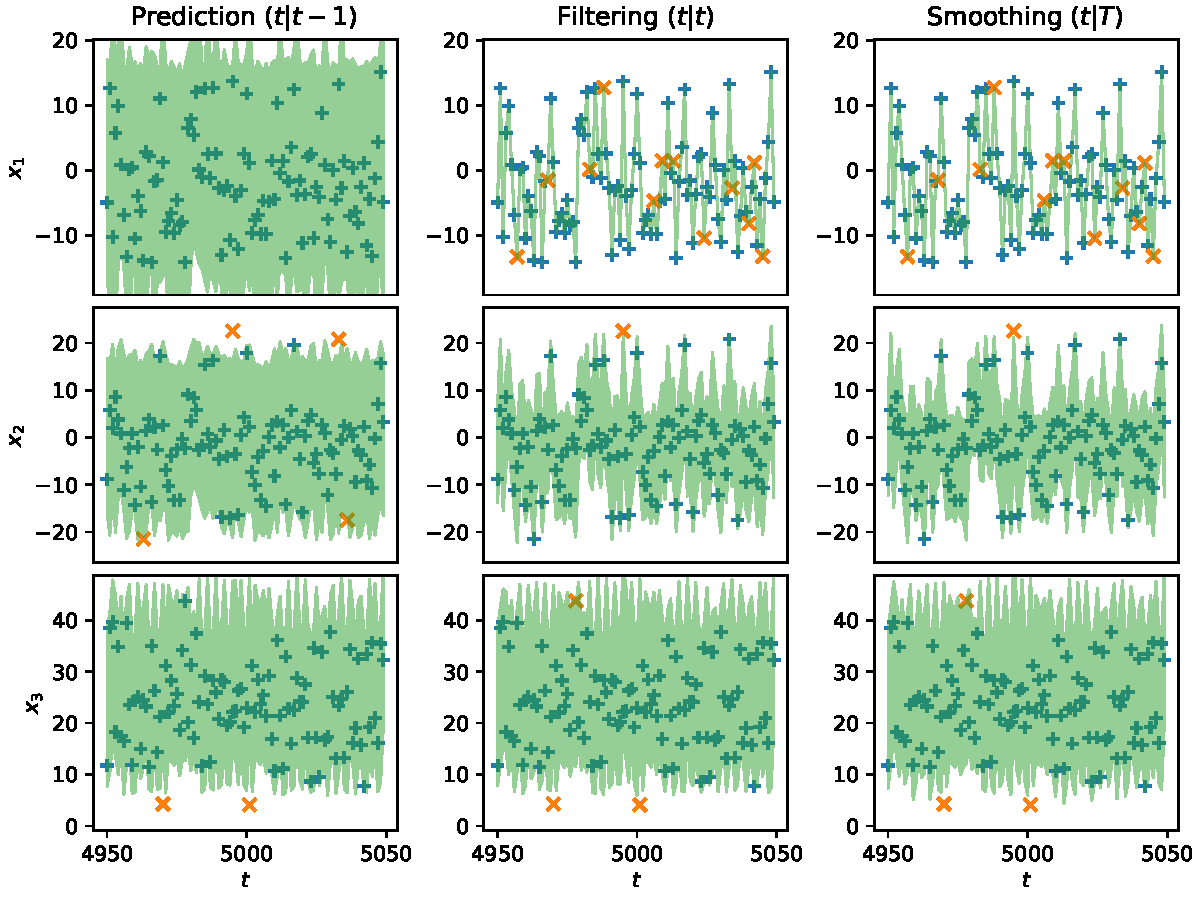
\includegraphics[width=\linewidth]{generated/trajectory/Method.ANALYTIC-Recalibrate.NO.pdf}
\end{center}
\caption{Trajectory excerpt for Kalman filter \textsc{{\textsc{analytic}}}}
\end{figure}
\begin{figure}[H]
\begin{center}
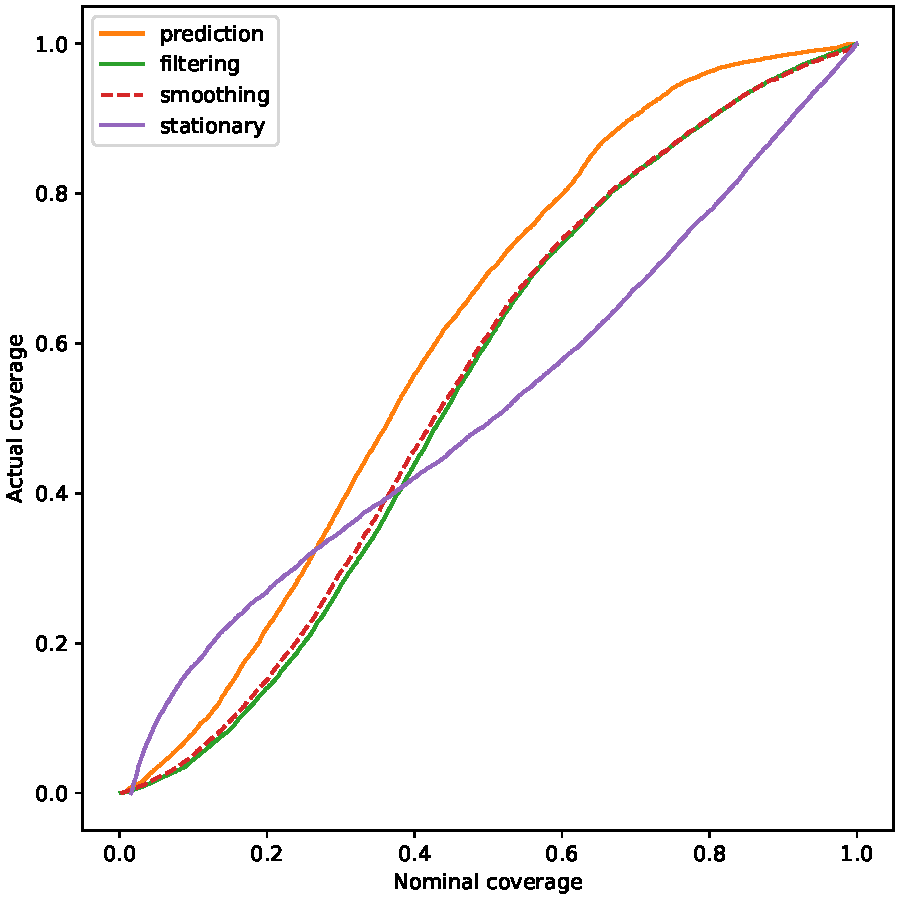
\includegraphics[width=\linewidth]{generated/coverage/Method.ANALYTIC-Recalibrate.NO.pdf}
\end{center}
\caption{Coverage for Kalman filter \textsc{{\textsc{analytic}}}}
\end{figure}
\subsection{Kalman Filter: {\textsc{analytic (recal)}}}
\begin{figure}[H]
\begin{center}
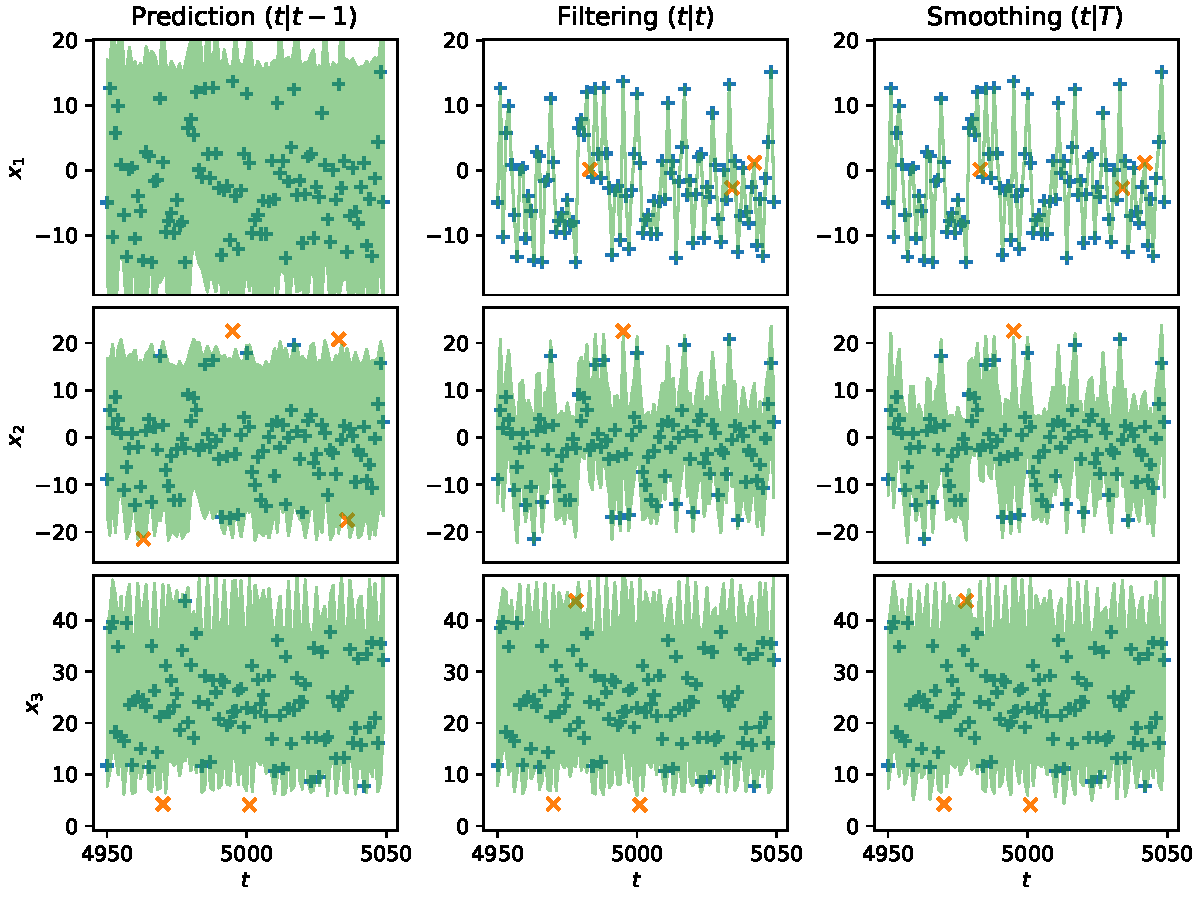
\includegraphics[width=\linewidth]{generated/trajectory/Method.ANALYTIC-Recalibrate.YES.pdf}
\end{center}
\caption{Trajectory excerpt for Kalman filter \textsc{{\textsc{analytic (recal)}}}}
\end{figure}
\begin{figure}[H]
\begin{center}
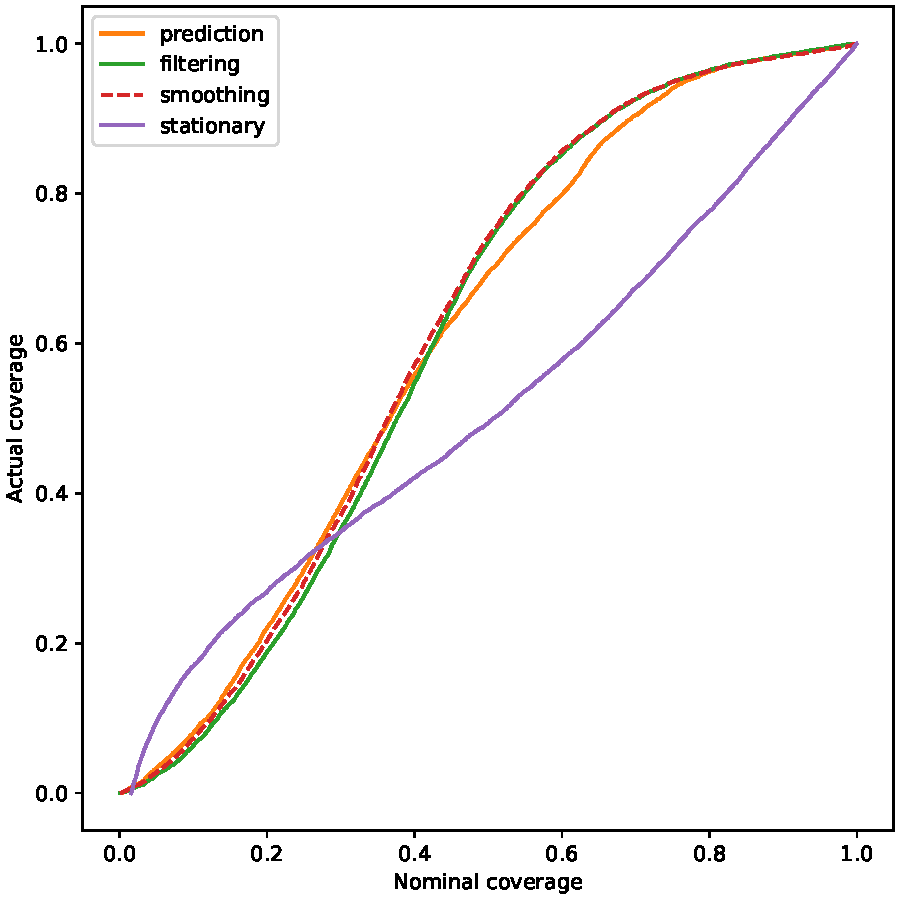
\includegraphics[width=\linewidth]{generated/coverage/Method.ANALYTIC-Recalibrate.YES.pdf}
\end{center}
\caption{Coverage for Kalman filter \textsc{{\textsc{analytic (recal)}}}}
\end{figure}
\subsection{Kalman Filter: {\textsc{mean-field}}}
\begin{figure}[H]
\begin{center}
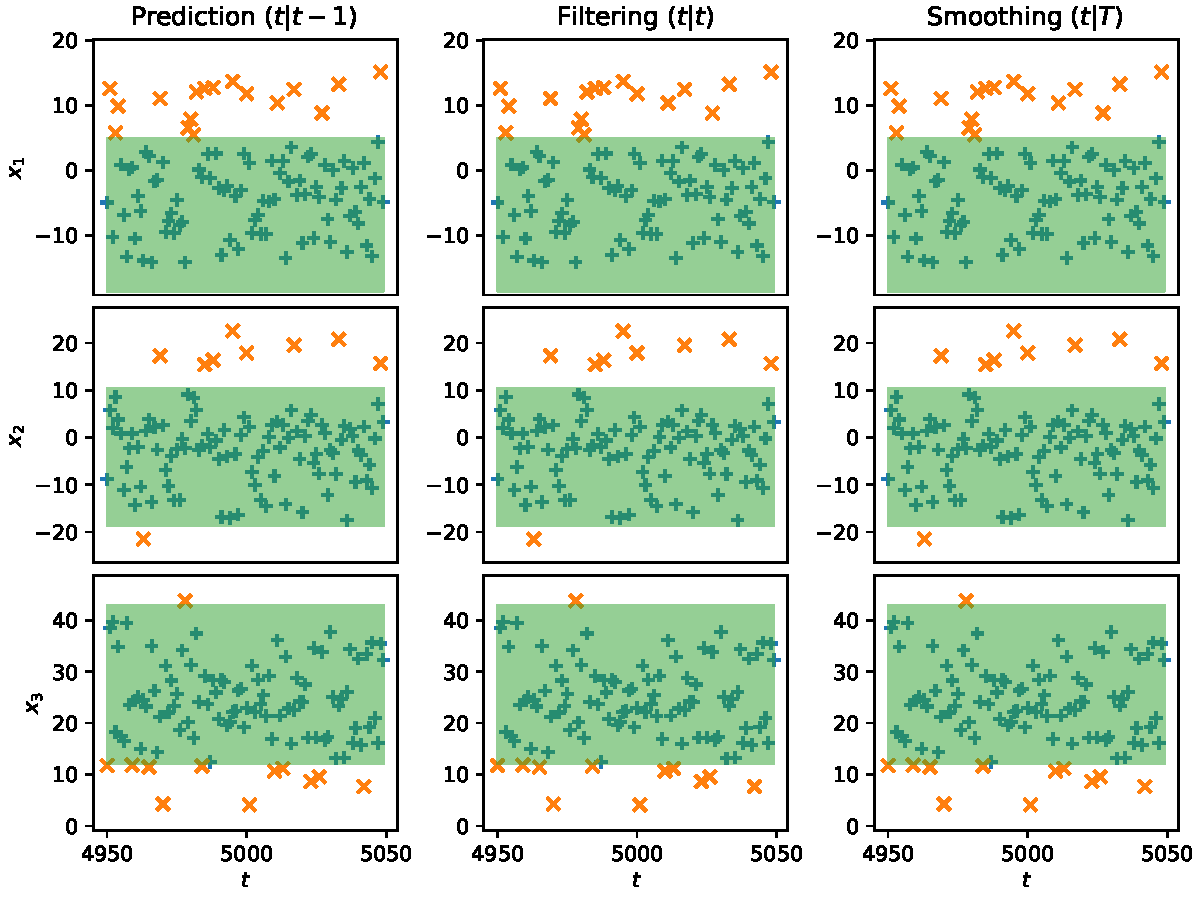
\includegraphics[width=\linewidth]{generated/trajectory/Method.MEAN_FIELD-Recalibrate.NO.pdf}
\end{center}
\caption{Trajectory excerpt for Kalman filter \textsc{{\textsc{mean-field}}}}
\end{figure}
\begin{figure}[H]
\begin{center}
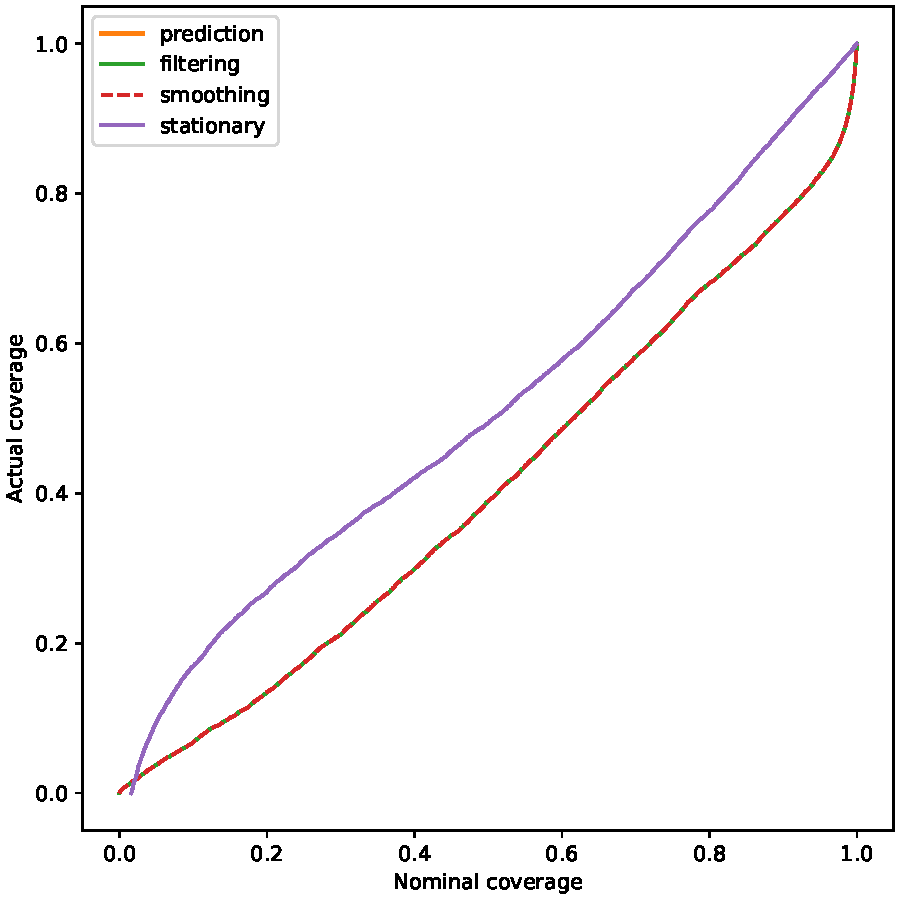
\includegraphics[width=\linewidth]{generated/coverage/Method.MEAN_FIELD-Recalibrate.NO.pdf}
\end{center}
\caption{Coverage for Kalman filter \textsc{{\textsc{mean-field}}}}
\end{figure}
\subsection{Kalman Filter: {\textsc{mean-field (recal)}}}
\begin{figure}[H]
\begin{center}
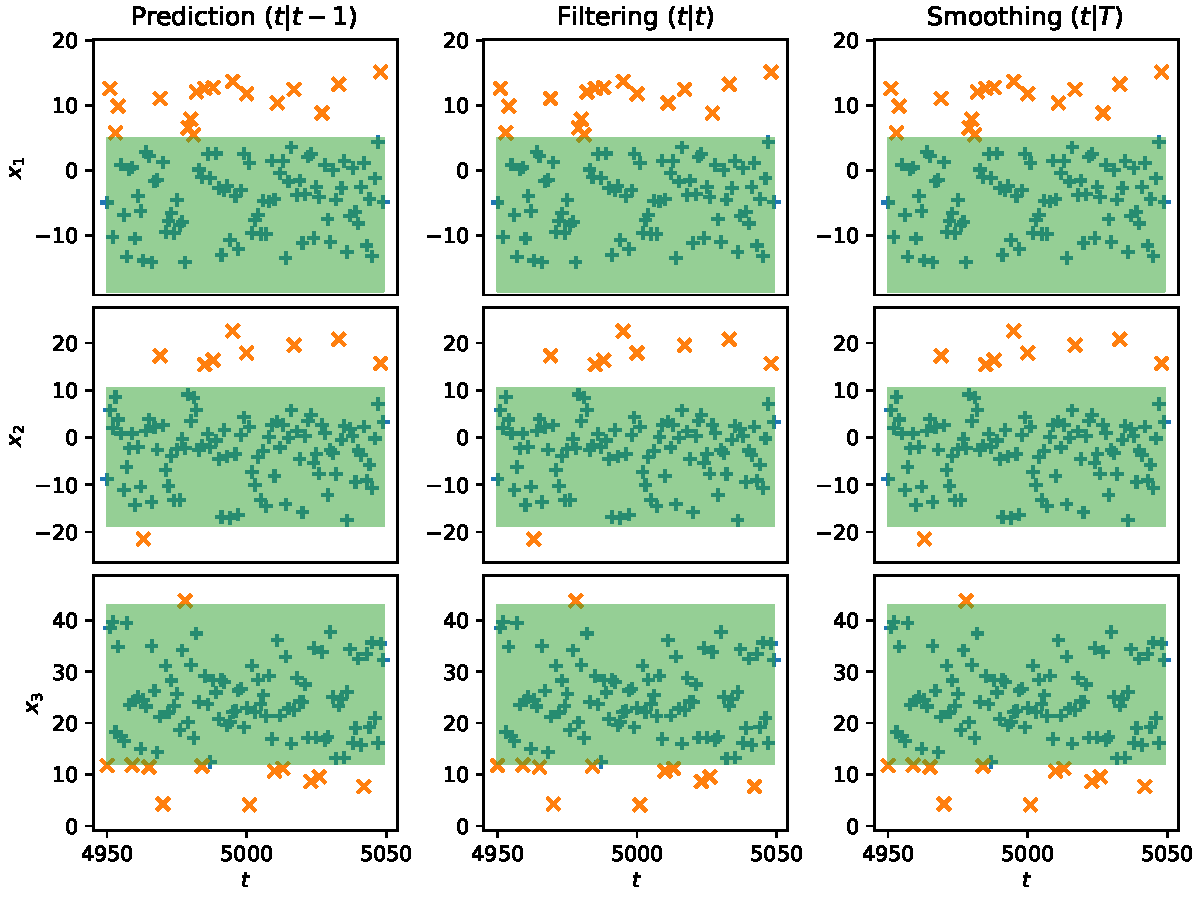
\includegraphics[width=\linewidth]{generated/trajectory/Method.MEAN_FIELD-Recalibrate.YES.pdf}
\end{center}
\caption{Trajectory excerpt for Kalman filter \textsc{{\textsc{mean-field (recal)}}}}
\end{figure}
\begin{figure}[H]
\begin{center}
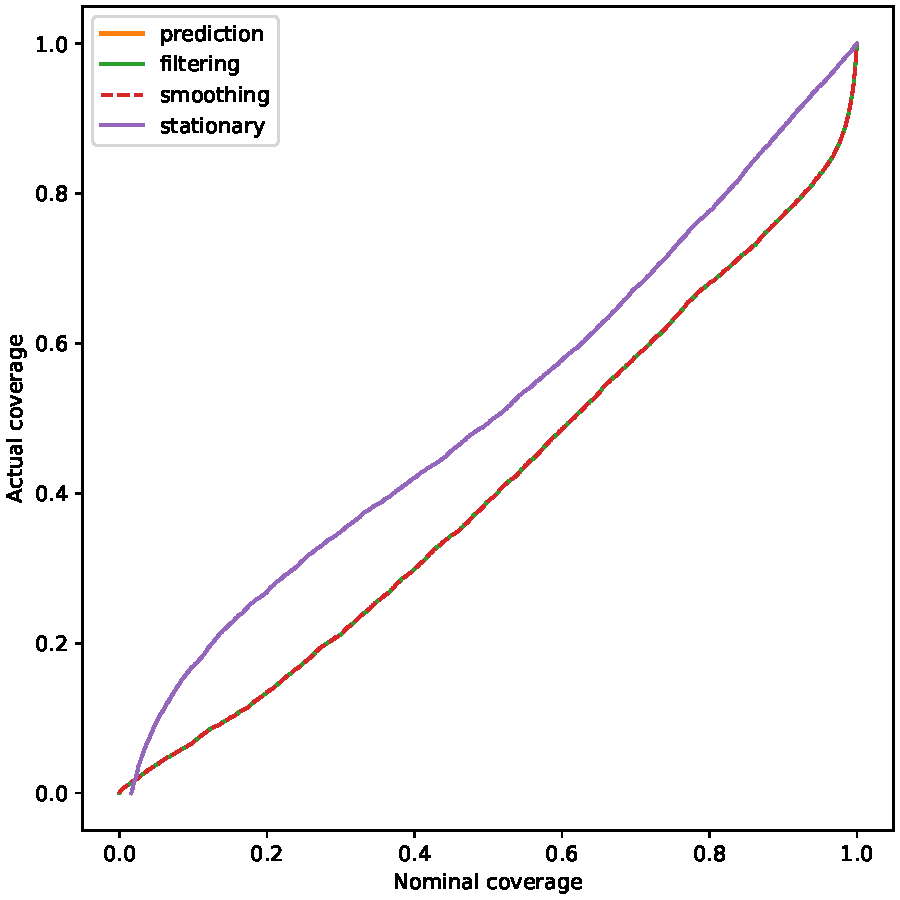
\includegraphics[width=\linewidth]{generated/coverage/Method.MEAN_FIELD-Recalibrate.YES.pdf}
\end{center}
\caption{Coverage for Kalman filter \textsc{{\textsc{mean-field (recal)}}}}
\end{figure}
\subsection{Kalman Filter: {\textsc{linear}}}
\begin{figure}[H]
\begin{center}
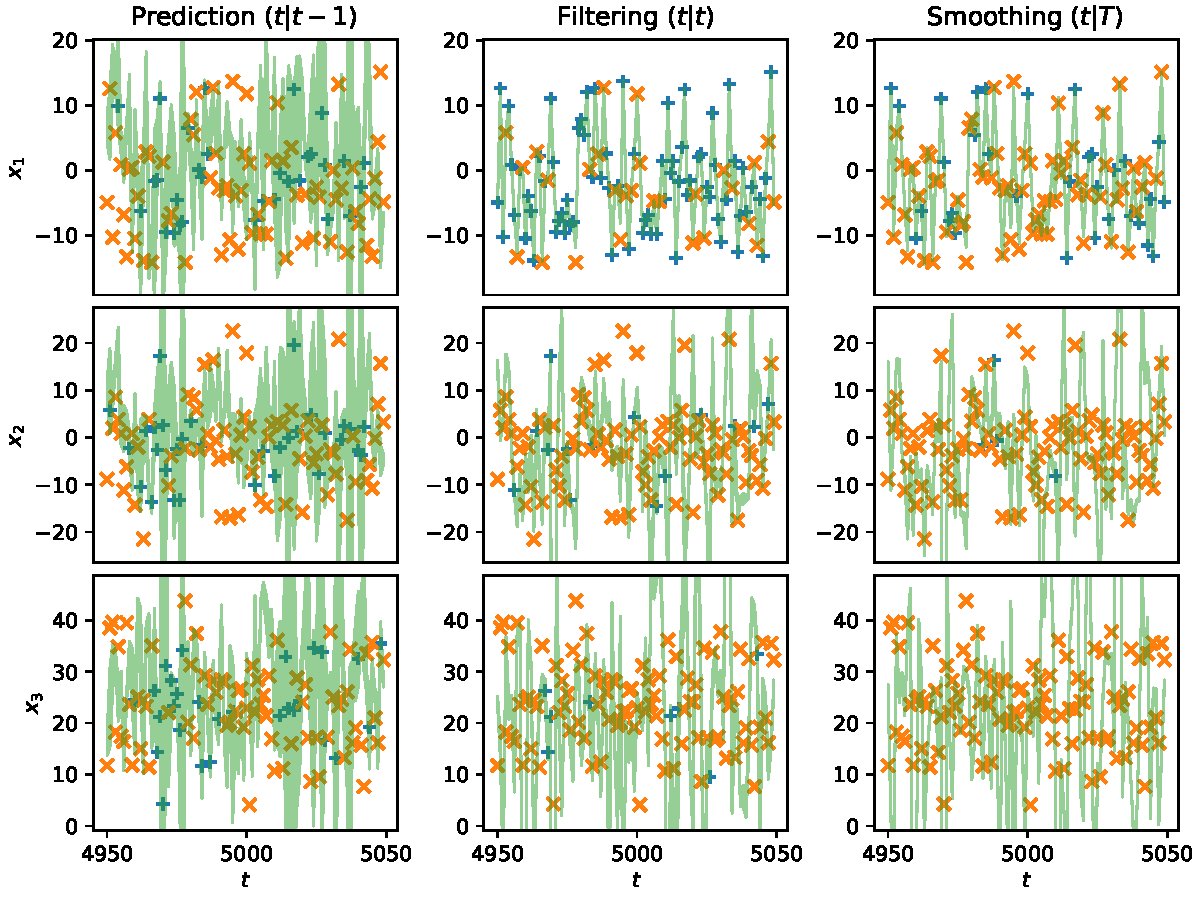
\includegraphics[width=\linewidth]{generated/trajectory/Method.LINEAR-Recalibrate.NO.pdf}
\end{center}
\caption{Trajectory excerpt for Kalman filter \textsc{{\textsc{linear}}}}
\end{figure}
\begin{figure}[H]
\begin{center}
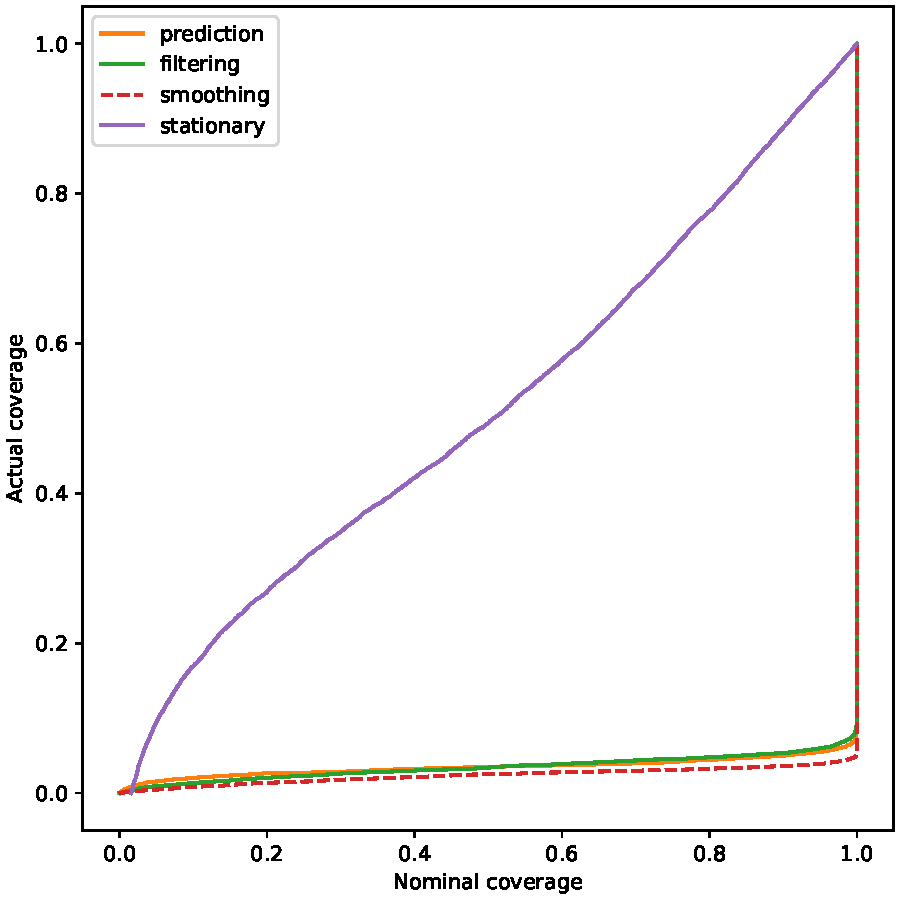
\includegraphics[width=\linewidth]{generated/coverage/Method.LINEAR-Recalibrate.NO.pdf}
\end{center}
\caption{Coverage for Kalman filter \textsc{{\textsc{linear}}}}
\end{figure}
\subsection{Kalman Filter: {\textsc{linear (recal)}}}
\begin{figure}[H]
\begin{center}
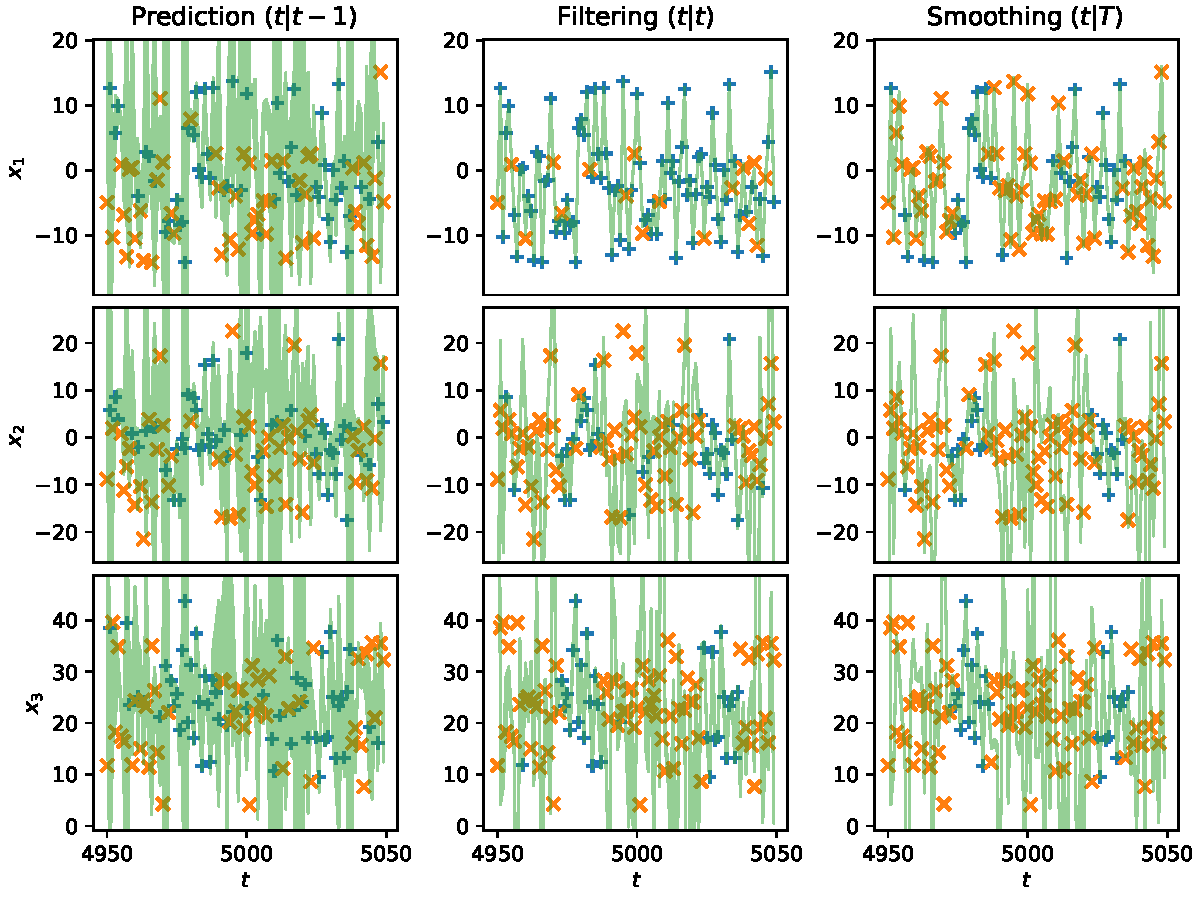
\includegraphics[width=\linewidth]{generated/trajectory/Method.LINEAR-Recalibrate.YES.pdf}
\end{center}
\caption{Trajectory excerpt for Kalman filter \textsc{{\textsc{linear (recal)}}}}
\end{figure}
\begin{figure}[H]
\begin{center}
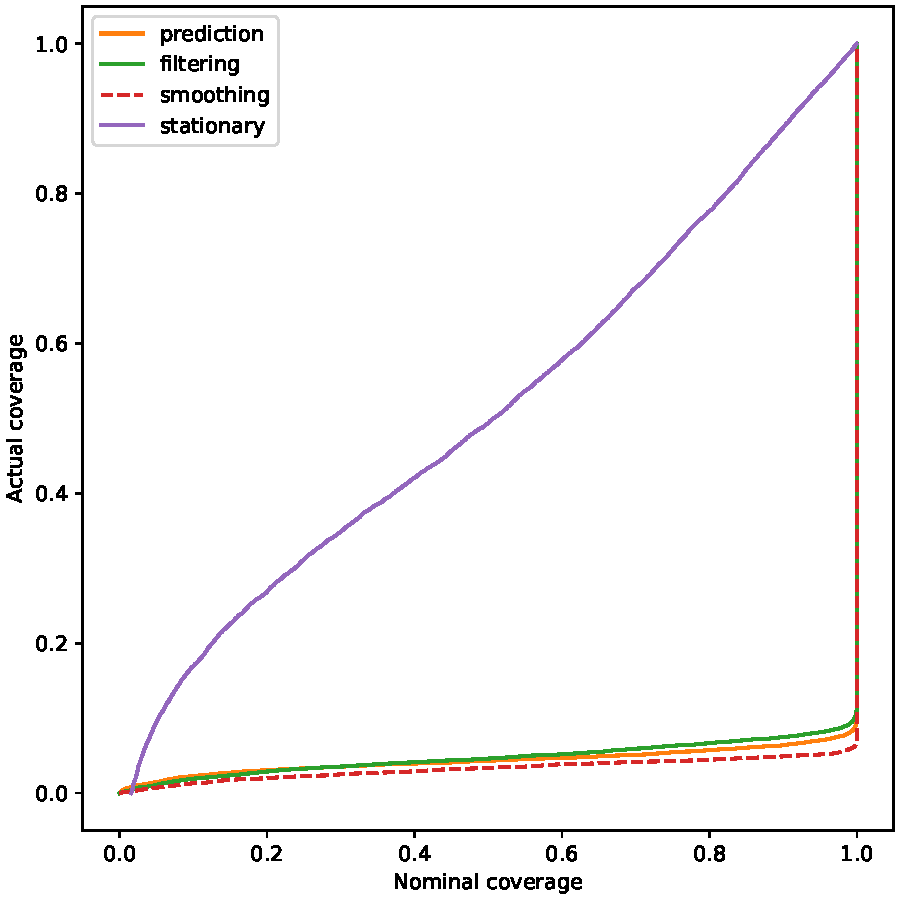
\includegraphics[width=\linewidth]{generated/coverage/Method.LINEAR-Recalibrate.YES.pdf}
\end{center}
\caption{Coverage for Kalman filter \textsc{{\textsc{linear (recal)}}}}
\end{figure}
\subsection{Kalman Filter: {\textsc{unscented'95}}}
\begin{figure}[H]
\begin{center}
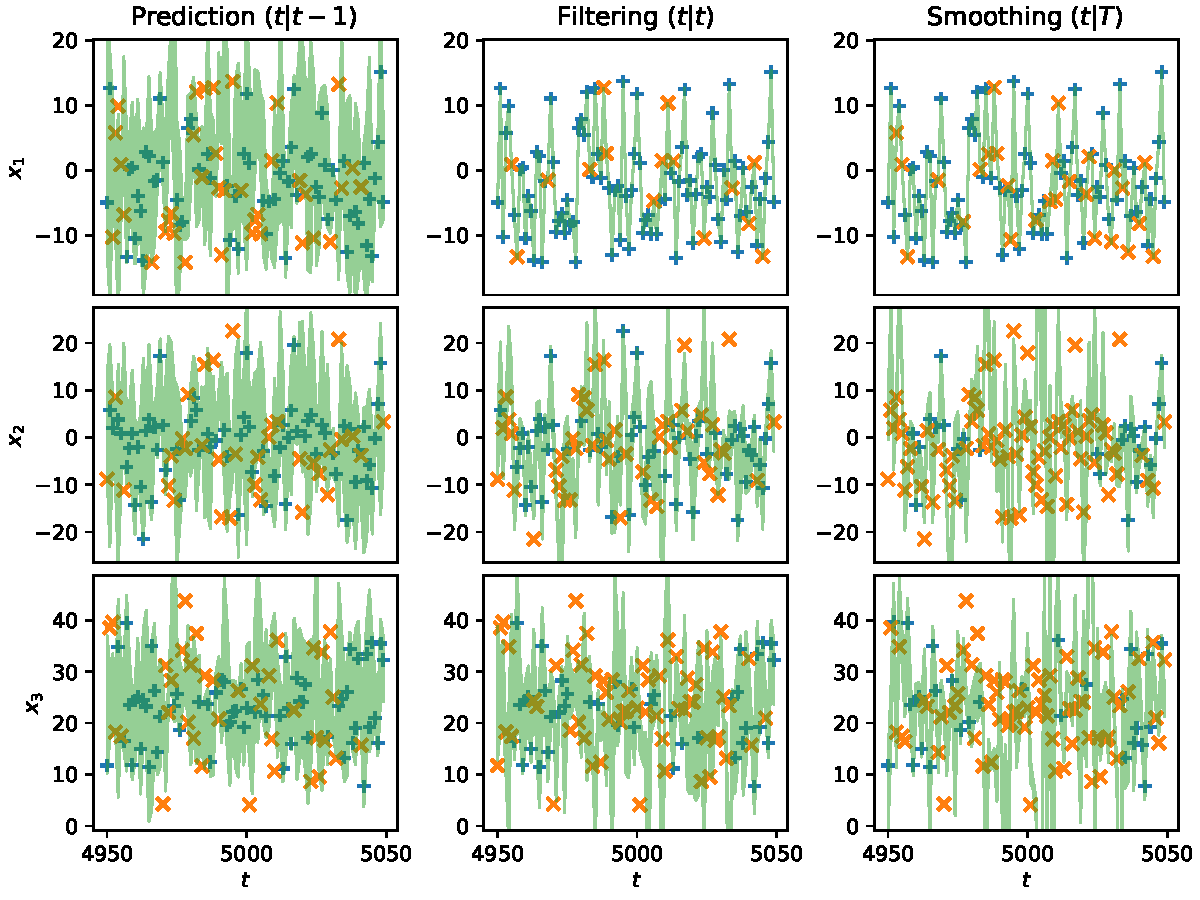
\includegraphics[width=\linewidth]{generated/trajectory/Method.UNSCENTED0-Recalibrate.NO.pdf}
\end{center}
\caption{Trajectory excerpt for Kalman filter \textsc{{\textsc{unscented'95}}}}
\end{figure}
\begin{figure}[H]
\begin{center}
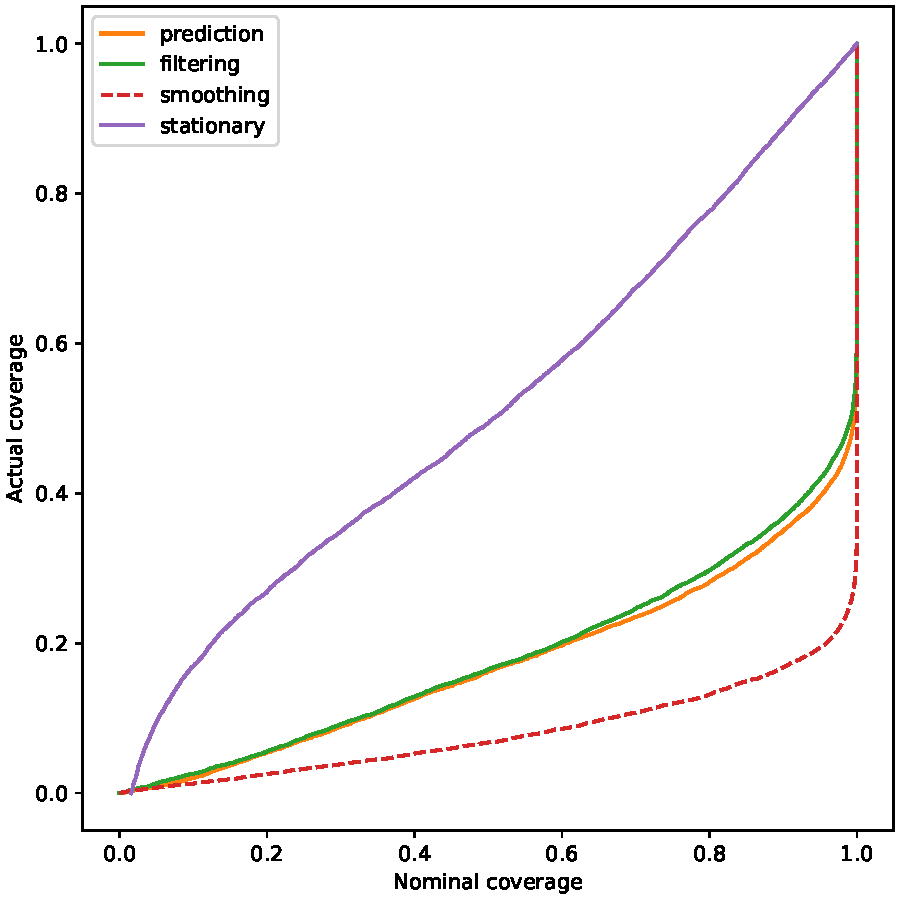
\includegraphics[width=\linewidth]{generated/coverage/Method.UNSCENTED0-Recalibrate.NO.pdf}
\end{center}
\caption{Coverage for Kalman filter \textsc{{\textsc{unscented'95}}}}
\end{figure}
\subsection{Kalman Filter: {\textsc{unscented'95 (recal)}}}
\begin{figure}[H]
\begin{center}
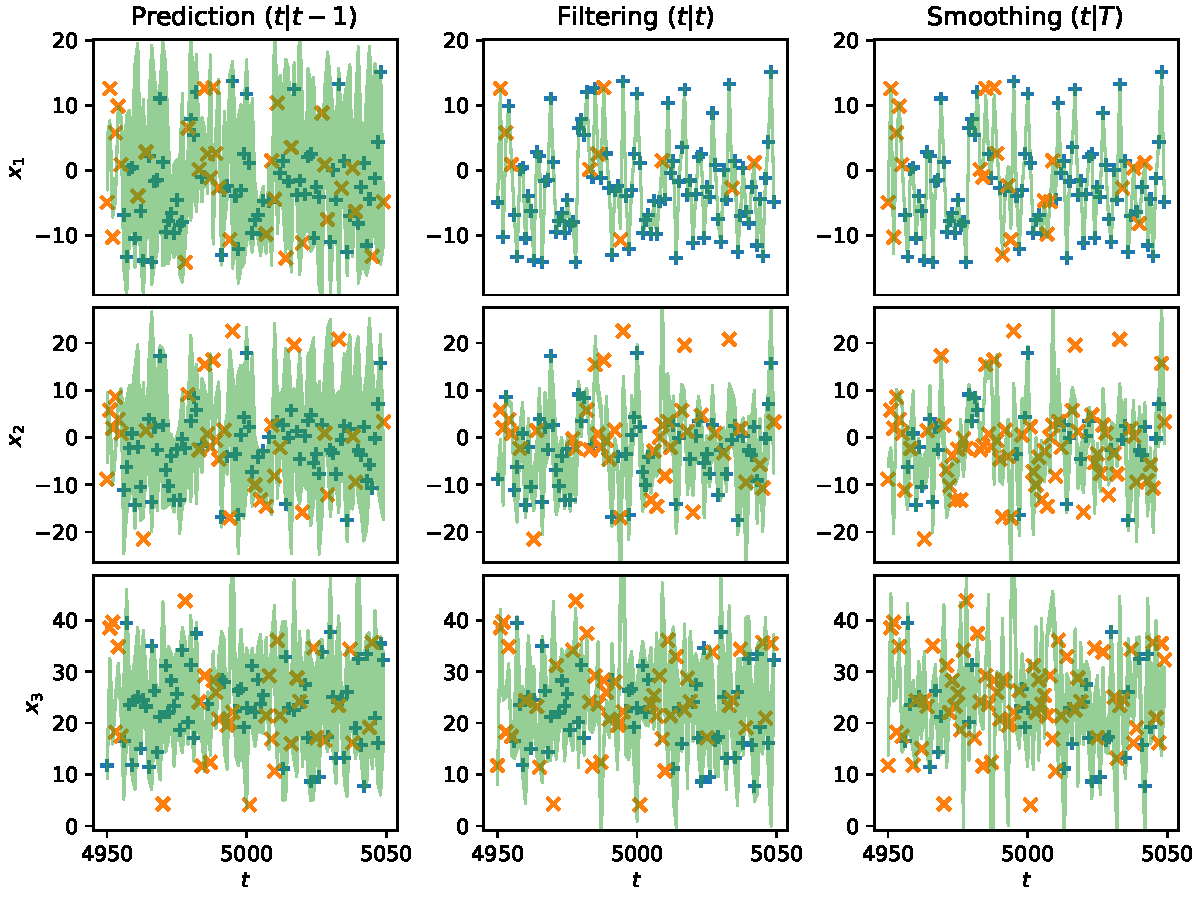
\includegraphics[width=\linewidth]{generated/trajectory/Method.UNSCENTED0-Recalibrate.YES.pdf}
\end{center}
\caption{Trajectory excerpt for Kalman filter \textsc{{\textsc{unscented'95 (recal)}}}}
\end{figure}
\begin{figure}[H]
\begin{center}
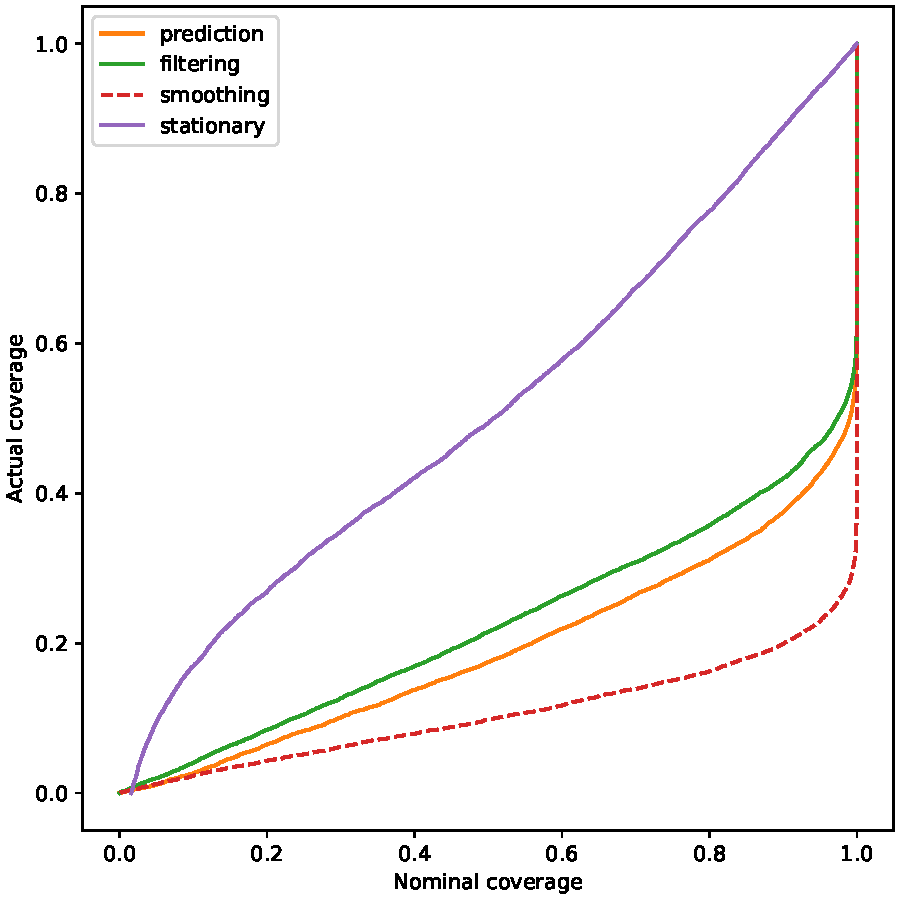
\includegraphics[width=\linewidth]{generated/coverage/Method.UNSCENTED0-Recalibrate.YES.pdf}
\end{center}
\caption{Coverage for Kalman filter \textsc{{\textsc{unscented'95 (recal)}}}}
\end{figure}
\subsection{Kalman Filter: {\textsc{unscented'02}}}
\begin{figure}[H]
\begin{center}
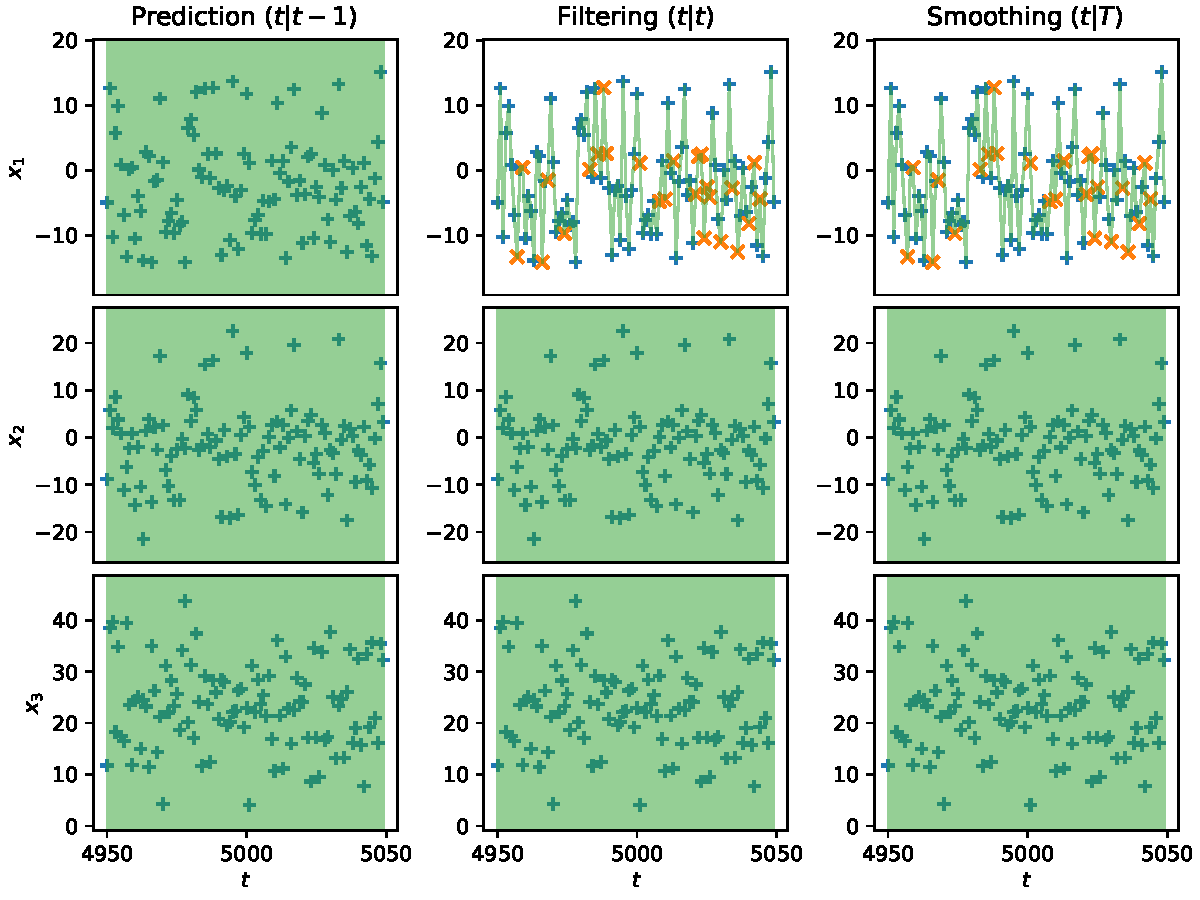
\includegraphics[width=\linewidth]{generated/trajectory/Method.UNSCENTED1-Recalibrate.NO.pdf}
\end{center}
\caption{Trajectory excerpt for Kalman filter \textsc{{\textsc{unscented'02}}}}
\end{figure}
\begin{figure}[H]
\begin{center}
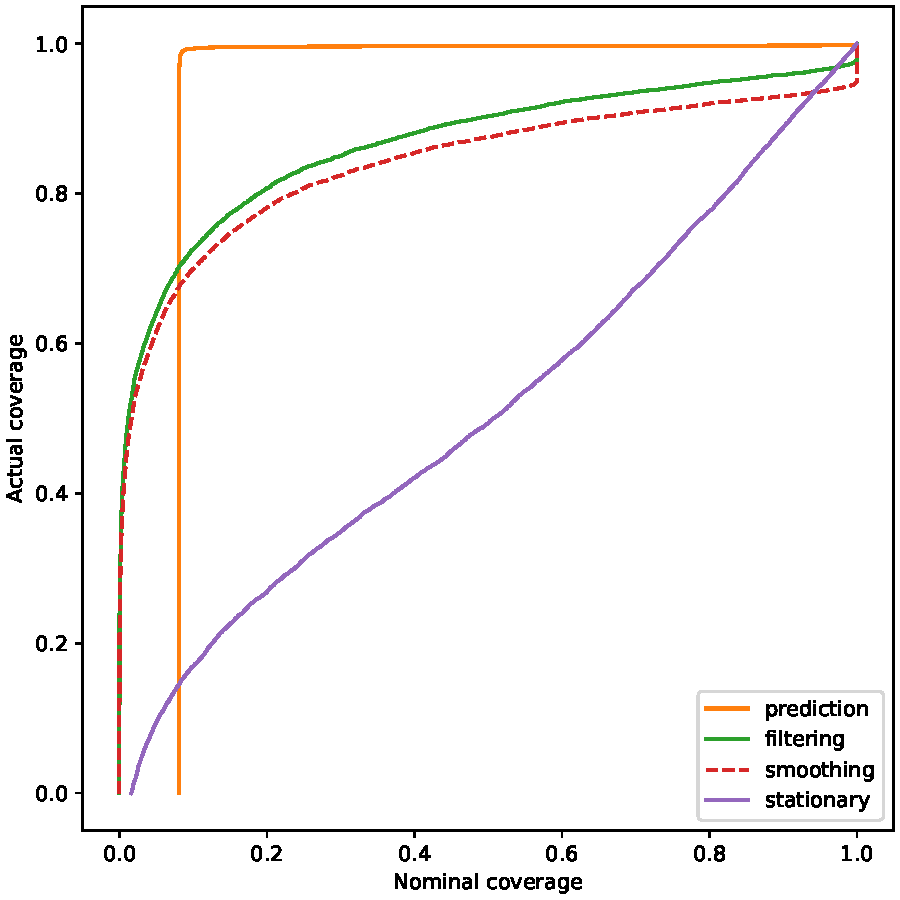
\includegraphics[width=\linewidth]{generated/coverage/Method.UNSCENTED1-Recalibrate.NO.pdf}
\end{center}
\caption{Coverage for Kalman filter \textsc{{\textsc{unscented'02}}}}
\end{figure}
\subsection{Kalman Filter: {\textsc{unscented'02 (recal)}}}
\begin{figure}[H]
\begin{center}
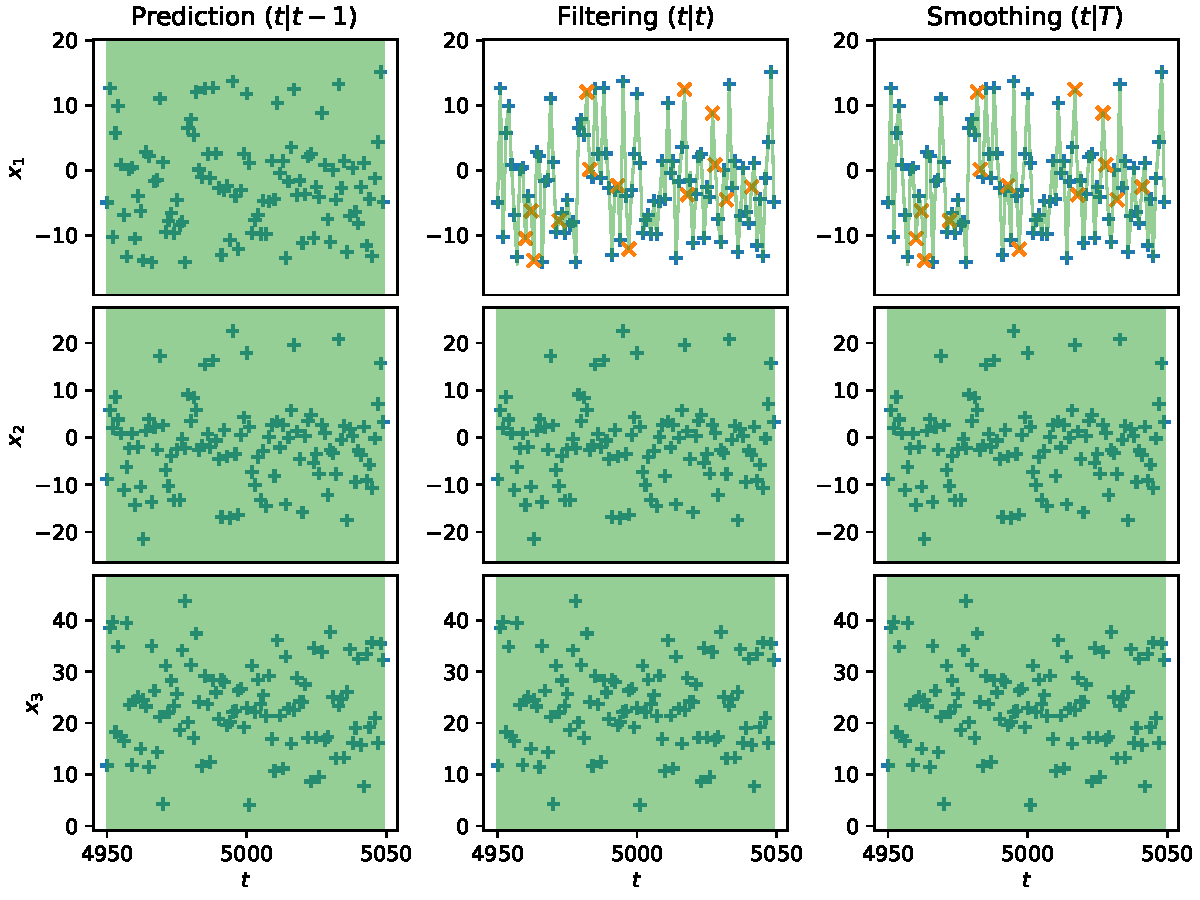
\includegraphics[width=\linewidth]{generated/trajectory/Method.UNSCENTED1-Recalibrate.YES.pdf}
\end{center}
\caption{Trajectory excerpt for Kalman filter \textsc{{\textsc{unscented'02 (recal)}}}}
\end{figure}
\begin{figure}[H]
\begin{center}
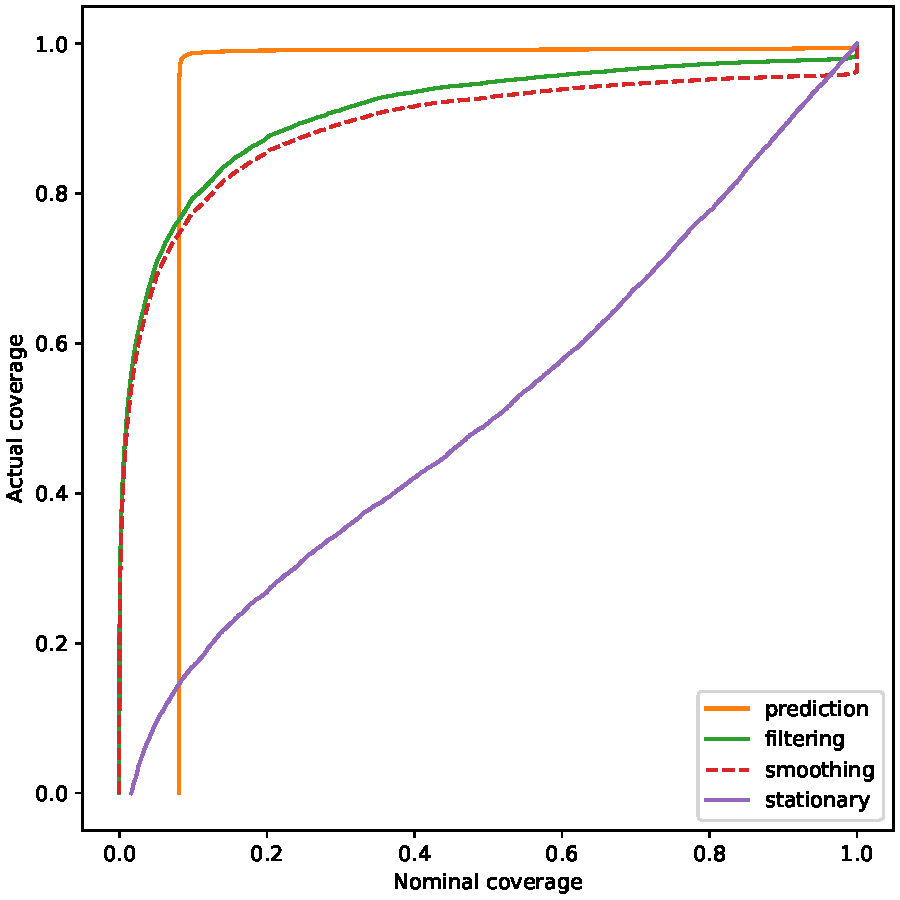
\includegraphics[width=\linewidth]{generated/coverage/Method.UNSCENTED1-Recalibrate.YES.pdf}
\end{center}
\caption{Coverage for Kalman filter \textsc{{\textsc{unscented'02 (recal)}}}}
\end{figure}


\end{document}
